%%**************************************************************
%% Vorlage fuer Bachelorarbeiten (o.ä.) der DHBW
%%
%% Autor: Tobias Dreher, Yves Fischer
%% Datum: 06.07.2011
%%
%% Autor: Michael Gruben
%% Datum: 15.05.2013
%%
%% Autor: Markus Barthel
%% Datum: 22.08.2014
%%**************************************************************

%!TEX root = ../dokumentation.tex

%
% Nahezu alle Einstellungen koennen hier getaetigt werden
%

\RequirePackage[l2tabu, orthodox]{nag}	% weist in Commandozeile bzw. log auf veraltete LaTeX Syntax hin

\documentclass[%
	pdftex,
	oneside,			% Einseitiger Druck.
	12pt,				% Schriftgroesse
	parskip=half,		% Halbe Zeile Abstand zwischen Absätzen.
%	topmargin = 10pt,	% Abstand Seitenrand (Std:1in) zu Kopfzeile [laut log: unused]
	headheight = 12pt,	% Höhe der Kopfzeile
%	headsep = 30pt,	% Abstand zwischen Kopfzeile und Text Body  [laut log: unused]
	headsepline,		% Linie nach Kopfzeile.
	footsepline,		% Linie vor Fusszeile.
	footheight = 16pt,	% Höhe der Fusszeile
	abstracton,		% Abstract Überschriften
	DIV=calc,		% Satzspiegel berechnen
	BCOR=8mm,		% Bindekorrektur links: 8mm
	headinclude=false,	% Kopfzeile nicht in den Satzspiegel einbeziehen
	footinclude=false,	% Fußzeile nicht in den Satzspiegel einbeziehen
	listof=totoc,		% Abbildungs-/ Tabellenverzeichnis im Inhaltsverzeichnis darstellen
	toc=bibliography,	% Literaturverzeichnis im Inhaltsverzeichnis darstellen
]{scrreprt}	% Koma-Script report-Klasse, fuer laengere Bachelorarbeiten alternativ auch: scrbook

% Einstellungen laden
\usepackage{xstring}
\usepackage[utf8]{inputenc}
\usepackage[T1]{fontenc}

\newcommand{\einstellung}[1]{%
  \expandafter\newcommand\csname #1\endcsname{}
  \expandafter\newcommand\csname setze#1\endcsname[1]{\expandafter\renewcommand\csname#1\endcsname{##1}}
}
\newcommand{\langstr}[1]{\einstellung{lang#1}}

\input{ads/einstellungen_liste} % verfügbare Einstellungen
%%%%%%%%%%%%%%%%%%%%%%%%%%%%%%%%%%%%%%%%%%%%%%%%%%%%%%%%%%%%%%%%%%%%%%%%%%%%%%%
%                                   Einstellungen
%
% Hier können alle relevanten Einstellungen für diese Arbeit gesetzt werden.
% Dazu gehören Angaben u.a. über den Autor sowie Formatierungen.
%
%
%%%%%%%%%%%%%%%%%%%%%%%%%%%%%%%%%%%%%%%%%%%%%%%%%%%%%%%%%%%%%%%%%%%%%%%%%%%%%%%


%%%%%%%%%%%%%%%%%%%%%%%%%%%%%%%%%%%% Sprache %%%%%%%%%%%%%%%%%%%%%%%%%%%%%%%%%%%
%% Aktuell sind Deutsch und Englisch unterstützt.
%% Es werden nicht nur alle vom Dokument erzeugten Texte in
%% der entsprechenden Sprache angezeigt, sondern auch weitere
%% Aspekte angepasst, wie z.B. die Anführungszeichen und
%% Datumsformate.
\setzesprache{de} % oder en
%%%%%%%%%%%%%%%%%%%%%%%%%%%%%%%%%%%%%%%%%%%%%%%%%%%%%%%%%%%%%%%%%%%%%%%%%%%%%%%%

%%%%%%%%%%%%%%%%%%%%%%%%%%%%%%%%%%% Angaben  %%%%%%%%%%%%%%%%%%%%%%%%%%%%%%%%%%%
%% Die meisten der folgenden Daten werden auf dem
%% Deckblatt angezeigt, einige auch im weiteren Verlauf
%% des Dokuments.
\setzematrikelnr{1234510}
\setzekurs{TINF17AIBI}
\setzetitel{Entwicklung einer KI für das Spiel Othello mithilfe des Algorithmus ProbCut}
\setzedatumAbgabe{29. April 2020}
\setzefirma{Firma GmbH}
\setzefirmenort{Firmenort}
\setzeabgabeort{Mannheim}
\setzeabschluss{Bachelor of Science}
\setzestudiengang{Angewandte Informatik}
\setzedhbw{Mannheim}
\setzebetreuer{Prof. Dr. Karl Stroetmann}
\setzegutachter{Dr.\ Silvana Koch-Mehrin}
\setzezeitraum{12 Wochen}
\setzearbeit{Studienarbeit}
\setzeautor{Paul Kupper und Thomas Möller}
%%%%%%%%%%%%%%%%%%%%%%%%%%%%%%%%%%%%%%%%%%%%%%%%%%%%%%%%%%%%%%%%%%%%%%%%%%%%%%%%

%%%%%%%%%%%%%%%%%%%%%%%%%%%% Literaturverzeichnis %%%%%%%%%%%%%%%%%%%%%%%%%%%%%%
%% Bei Fehlern während der Verarbeitung bitte in ads/header.tex bei der
%% Einbindung des Pakets biblatex (ungefähr ab Zeile 110,
%% einmal für jede Sprache), biber in bibtex ändern.
\newcommand{\ladeliteratur}{%
\addbibresource{bibliographie.bib}
%\addbibresource{weitereDatei.bib}
}
%% Zitierstil
%% siehe: http://ctan.mirrorcatalogs.com/macros/latex/contrib/biblatex/doc/biblatex.pdf (3.3.1 Citation Styles)
%% mögliche Werte z.B numeric-comp, alphabetic, authoryear
\setzezitierstil{alphabetic}
%%%%%%%%%%%%%%%%%%%%%%%%%%%%%%%%%%%%%%%%%%%%%%%%%%%%%%%%%%%%%%%%%%%%%%%%%%%%%%%%

%%%%%%%%%%%%%%%%%%%%%%%%%%%%%%%%% Layout %%%%%%%%%%%%%%%%%%%%%%%%%%%%%%%%%%%%%%%
%% Verschiedene Schriftarten
% laut nag Warnung: palatino obsolete, use mathpazo, helvet (option scaled=.95), courier instead
\setzeschriftart{lmodern} % palatino oder goudysans, lmodern, libertine

%% Paket um Textteile drehen zu können
%\usepackage{rotating}
%% Paket um Seite im Querformat anzuzeigen
%\usepackage{lscape}

%% Seitenränder
\setzeseitenrand{2.5cm}

%% Abstand vor Kapitelüberschriften zum oberen Seitenrand
\setzekapitelabstand{20pt}

%% Spaltenabstand
\setzespaltenabstand{10pt}
%%Zeilenabstand innerhalb einer Tabelle
\setzezeilenabstand{1.5}
%%%%%%%%%%%%%%%%%%%%%%%%%%%%%%%%%%%%%%%%%%%%%%%%%%%%%%%%%%%%%%%%%%%%%%%%%%%%%%%%

%%%%%%%%%%%%%%%%%%%%%%%%%%%%% Verschiedenes  %%%%%%%%%%%%%%%%%%%%%%%%%%%%%%%%%%%
%% Farben (Angabe in HTML-Notation mit großen Buchstaben)
\newcommand{\ladefarben}{%
	\definecolor{LinkColor}{HTML}{00007A}
	\definecolor{ListingBackground}{HTML}{FCF7DE}
    \definecolor{lightergray}{gray}{0.95}
}
%% Mathematikpakete benutzen (Pakete aktivieren)
%\usepackage{amsmath}
%\usepackage{amssymb}

%% Programmiersprachen Highlighting (Listings)
\newcommand{\listingsettings}{%
	\lstset{%
		language=Java,			% Standardsprache des Quellcodes
		numbers=left,			% Zeilennummern links
		stepnumber=1,			% Jede Zeile nummerieren.
		numbersep=5pt,			% 5pt Abstand zum Quellcode
		numberstyle=\tiny,		% Zeichengrösse 'tiny' für die Nummern.
		breaklines=true,		% Zeilen umbrechen wenn notwendig.
		breakautoindent=true,	% Nach dem Zeilenumbruch Zeile einrücken.
		postbreak=\space,		% Bei Leerzeichen umbrechen.
		tabsize=2,				% Tabulatorgrösse 2
		basicstyle=\ttfamily\footnotesize, % Nichtproportionale Schrift, klein für den Quellcode
		showspaces=false,		% Leerzeichen nicht anzeigen.
		showstringspaces=false,	% Leerzeichen auch in Strings ('') nicht anzeigen.
		extendedchars=true,		% Alle Zeichen vom Latin1 Zeichensatz anzeigen.
		captionpos=b,			% sets the caption-position to bottom
		backgroundcolor=\color{ListingBackground}, % Hintergrundfarbe des Quellcodes setzen.
		xleftmargin=0pt,		% Rand links
		xrightmargin=0pt,		% Rand rechts
		frame=single,			% Rahmen an
		frameround=ffff,
		rulecolor=\color{darkgray},	% Rahmenfarbe
		fillcolor=\color{ListingBackground},
		keywordstyle=\color[rgb]{0.133,0.133,0.6},
		commentstyle=\color[rgb]{0.133,0.545,0.133},
		stringstyle=\color[rgb]{0.627,0.126,0.941}
	}
}
%%%%%%%%%%%%%%%%%%%%%%%%%%%%%%%%%%%%%%%%%%%%%%%%%%%%%%%%%%%%%%%%%%%%%%%%%%%%%%%%

%%%%%%%%%%%%%%%%%%%%%%%%%%%%%%%% Eigenes %%%%%%%%%%%%%%%%%%%%%%%%%%%%%%%%%%%%%%%
%% Hier können Ergänzungen zur Präambel vorgenommen werden (eigene Pakete, Einstellungen)

\newcommand{\passthrough}[1]{\lstset{mathescape=false}#1\lstset{mathescape=true}}

 % lese Einstellungen

\input{lang/strings} % verfügbare Strings
\input{lang/\sprache} % Übersetzung einlesen

% Einstellung der Sprache des Paketes Babel und der Verzeichnisüberschriften
\iflang{de}{\usepackage[english, ngerman]{babel}}
\iflang{en}{\usepackage[ngerman, english]{babel}} 


%%%%%%% Package Includes %%%%%%%

\usepackage[margin=\seitenrand,foot=1cm]{geometry}	% Seitenränder und Abstände
\usepackage[activate]{microtype} %Zeilenumbruch und mehr
\usepackage[onehalfspacing]{setspace}
\usepackage{makeidx}
\usepackage[autostyle=true,german=quotes]{csquotes}
\usepackage{longtable}
\usepackage{enumitem}	% mehr Optionen bei Aufzählungen
\usepackage{graphicx}
\usepackage{pdfpages}   % zum Einbinden von PDFs
\usepackage{xcolor} 	% für HTML-Notation
\usepackage{float}
\usepackage{array}
\usepackage{calc}		% zum Rechnen (Bildtabelle in Deckblatt)
\usepackage[right]{eurosym}
\usepackage{wrapfig}
\usepackage{pgffor} % für automatische Kapiteldateieinbindung
\usepackage[perpage, hang, multiple, stable]{footmisc} % Fussnoten
\usepackage[printonlyused]{acronym} % falls gewünscht kann die Option footnote eingefügt werden, dann wird die Erklärung nicht inline sondern in einer Fußnote dargestellt
\usepackage{listings}
\usepackage{minted}
\usepackage{tikz}
\usepackage{tikz-qtree}
\usetikzlibrary{shapes.geometric}
\usetikzlibrary{positioning}

% Notizen. Einsatz mit \todo{Notiz} oder \todo[inline]{Notiz}. 
\usepackage[obeyFinal,backgroundcolor=yellow,linecolor=black]{todonotes}
% Alle Notizen ausblenden mit der Option "final" in \documentclass[...] oder durch das auskommentieren folgender Zeile
% \usepackage[disable]{todonotes}

% Kommentarumgebung. Einsatz mit \comment{}. Alle Kommentare ausblenden mit dem Auskommentieren der folgenden und dem aktivieren der nächsten Zeile.
\newcommand{\comment}[1]{\par {\bfseries \color{blue} #1 \par}} %Kommentar anzeigen
% \newcommand{\comment}[1]{} %Kommentar ausblenden


%%%%%% Configuration %%%%%

%% Anwenden der Einstellungen

\usepackage{\schriftart}
\ladefarben{}

% Titel, Autor und Datum
\title{\titel}
\author{\autor}
\date{\datum}

% PDF Einstellungen
\usepackage[%
	pdftitle={\titel},
	pdfauthor={\autor},
	pdfsubject={\arbeit},
	pdfcreator={pdflatex, LaTeX with KOMA-Script},
	pdfpagemode=UseOutlines, 		% Beim Oeffnen Inhaltsverzeichnis anzeigen
	pdfdisplaydoctitle=true, 		% Dokumenttitel statt Dateiname anzeigen.
	pdflang={\sprache}, 			% Sprache des Dokuments.
]{hyperref}

\usepackage{caption}

% (Farb-)einstellungen für die Links im PDF
\hypersetup{%
	colorlinks=true, 		% Aktivieren von farbigen Links im Dokument
	linkcolor=LinkColor, 	% Farbe festlegen
	citecolor=LinkColor,
	filecolor=LinkColor,
	menucolor=LinkColor,
	urlcolor=LinkColor,
	linktocpage=true, 		% Nicht der Text sondern die Seitenzahlen in Verzeichnissen klickbar
	bookmarksnumbered=true 	% Überschriftsnummerierung im PDF Inhalt anzeigen.
}
% Workaround um Fehler in Hyperref, muss hier stehen bleiben
\usepackage{bookmark} %nur ein latex-Durchlauf für die Aktualisierung von Verzeichnissen nötig

% Schriftart in Captions etwas kleiner
\addtokomafont{caption}{\small}

% Literaturverweise (sowohl deutsch als auch englisch)
\iflang{de}{%
\usepackage[
	backend=biber,		% empfohlen. Falls biber Probleme macht: bibtex
	bibwarn=true,
	bibencoding=utf8,	% wenn .bib in utf8, sonst ascii
	sortlocale=de_DE,
	style=\zitierstil,
]{biblatex}
}
\iflang{en}{%
\usepackage[
	backend=biber,		% empfohlen. Falls biber Probleme macht: bibtex
	bibwarn=true,
	bibencoding=utf8,	% wenn .bib in utf8, sonst ascii
	sortlocale=en_US,
	style=\zitierstil,
]{biblatex}
}

\ladeliteratur{}

% Glossar
\usepackage[nonumberlist,toc]{glossaries}

%%%%%% Additional settings %%%%%%

% Hurenkinder und Schusterjungen verhindern
% http://projekte.dante.de/DanteFAQ/Silbentrennung
\clubpenalty = 10000 % schließt Schusterjungen aus (Seitenumbruch nach der ersten Zeile eines neuen Absatzes)
\widowpenalty = 10000 % schließt Hurenkinder aus (die letzte Zeile eines Absatzes steht auf einer neuen Seite)
\displaywidowpenalty=10000

% Bildpfad
\graphicspath{{images/}}

% Einige häufig verwendete Sprachen
\lstloadlanguages{Python,bash}
\listingsettings{}
% Umbennung des Listings
\renewcommand\lstlistingname{\langlistingname}
\renewcommand\lstlistlistingname{\langlistlistingname}
\def\lstlistingautorefname{\langlistingautorefname}

% Abstände in Tabellen
\setlength{\tabcolsep}{\spaltenabstand}
\renewcommand{\arraystretch}{\zeilenabstand}


\makeglossaries
\input{ads/glossary}

\begin{document}

	% Deckblatt
	\begin{spacing}{1}
		%!TEX root = ../dokumentation.tex

\begin{titlepage}
	\begin{longtable}{p{8.2cm} p{5.4cm}} %TODO: center
		{\raisebox{\ht\strutbox-\totalheight}{\includegraphics[height=2.5cm]{images/dhbw.png}}}
	\end{longtable}
	\enlargethispage{20mm}
	\begin{center}
		\vspace*{12mm}	{\LARGE\textbf \titel }\\
		\vspace*{12mm}	{\large\textbf \arbeit}\\
		%\vspace*{12mm}	\langdeckblattabschlusshinleitung\\
		%\vspace*{3mm}		{\textbf \abschluss}\\
		\vspace*{12mm}	\langartikelstudiengang{} \langstudiengang{} \studiengang\\
    \vspace*{3mm}		\langanderdh{} \dhbw\\
		\vspace*{12mm}	\langvon\\
		\vspace*{3mm}		{\large\textbf \autor}\\
		\vspace*{12mm}	\datumAbgabe\\
	\end{center}
	\vfill
	\begin{spacing}{1.2}
	\begin{tabbing}
		mmmmmmmmmmmmmmmmmmmmmmmmmm             \= \kill
		\textbf{\langdbbearbeitungszeit}       \>  \zeitraum\\
		\textbf{\langdbkurs}  \>  \kurs\\
		%\textbf{\langdbfirma}                  \>  \firma, \firmenort\\
		\textbf{\langdbbetreuer}               \>  \betreuer\\
		%\textbf{\langdbgutachter}              \>  \gutachter
	\end{tabbing}
	\end{spacing}
\end{titlepage}

	\end{spacing}
	\newpage

	\pagenumbering{Roman}

	% Sperrvermerk
	%\input{ads/sperrvermerk}
	%\newpage

	% Erklärung
	%!TEX root = ../dokumentation.tex

\thispagestyle{empty}

\section*{\langerklaerung}
\vspace*{2em}

\iflang{de}{%
Wir versichern hiermit, dass wir unsere {\arbeit} mit dem Thema: {\itshape \titel } selbstständig verfasst und keine anderen als die angegebenen Quellen und Hilfsmittel benutzt haben. Wir versichern zudem, dass die eingereichte elektronische Fassung mit der gedruckten Fassung übereinstimmt. 

% https://www.dhbw-karlsruhe.de/fileadmin/user_upload/dokumente/T-Informatik/Prüfungsordnung-Technik-2015-09-29.pdf (S. 19)
% https://www.dhbw-stuttgart.de/fileadmin/dateien/Amtliche_Bekanntmachungen/20_2017_Bekanntmachung_StuPrO_DHBW_Technik.pdf (S. 21)


% Ich erkläre hiermit ehrenwörtlich: \\
% \begin{enumerate}
% \item dass ich meine {\arbeit} mit dem Thema
% {\itshape \titel } ohne fremde Hilfe angefertigt habe;
% \item dass ich die Übernahme wörtlicher Zitate aus der Literatur sowie die Verwendung der Gedanken
% anderer Autoren an den entsprechenden Stellen innerhalb der Arbeit gekennzeichnet habe;
% \item dass ich meine {\arbeit} bei keiner anderen Prüfung vorgelegt habe;
% \item dass die eingereichte elektronische Fassung exakt mit der eingereichten schriftlichen Fassung
% übereinstimmt.
% \end{enumerate}
% 
% Ich bin mir bewusst, dass eine falsche Erklärung rechtliche Folgen haben wird.

% % http://www.ib.dhbw-mannheim.de/fileadmin/ms/bwl-ib/Downloads_alt/Leitfaden_31.05.pdf (S. 52)
}


\iflang{en}{%
Hereby I solemnly declare:
\begin{enumerate}
\item that this {\arbeit}, titled {\itshape \titel } is entirely the product of my own scholarly work, unless otherwise indicated in the text or references, or acknowledged below;
\item I have indicated the thoughts adopted directly or indirectly from other sources at the appropriate places within the document;
\item this {\arbeit} has not been submitted either in whole or part, for a degree at this or any other university or institution;
\item I have not published this {\arbeit} in the past; 
\item the printed version is equivalent to the submitted electronic one.
\end{enumerate}
I am aware that a dishonest declaration will entail legal consequences.
}

\vspace{3em}

\abgabeort, \datumAbgabe
\vspace{4em}

\rule{6cm}{0.4pt}\\
\autor

	\newpage

	% Abstract
	%%!TEX root = ../dokumentation.tex

\pagestyle{empty}

\renewcommand{\abstractname}{\langabstract}

\begin{otherlanguage}{english}
\begin{abstract}
Othello is a board game for two players. Due to the games deterministic nature, the strength of a player is solely
determined by their decision making and strategy.

The goal of this research project is to develop an artificial intelligence for the game Othello, which aims to be as
strong as possible, ideally beating human players as well as some publicly available AI agents. This
artificial intelligence is to be implemented as a Jupyter Notebook in the Python programming language, and can be played
against by a human player using a graphical interface.

The Minimax algorithm with depth-limited search and a heuristic for evaluating game states serves as a base for the
implementation. Alpha-beta pruning and the probabilistic forward cuts of ProbCut further optimize the performance and hence the strength of this algorithm. In addition, different features for use in the heuristic
function are tested and weighted.

The result of this project is a highly configurable artificial intelligence, that consistently wins against publicly
available AIs such as cowthello and two agents developed as part of a predecessor project. The AI is comfortably
configurable and usable through the user interface implemented in the Jupyter Notebook.

\end{abstract}
\end{otherlanguage}


\renewcommand{\abstractname}{\langabstract}

\begin{abstract}
Othello ist ein Brettspiel, welches von zwei Spielern gespielt wird. Da das Spiel völlig deterministisch ist, wird die
Stärke eines Spielers einzig und allein von dessen Entscheidungen und somit dessen Strategie bestimmt.

Ziel dieser Arbeit ist es, eine möglichst starke Künstliche Intelligenz für das Spiel Othello zu entwickeln, die sowohl
gegen menschliche Spieler als auch gegen einige öffentlich verfügbare KI-Agenten gewinnt. Die Implementierung findet in Form
eines Jupyter Notebooks in der Programmiersprache Python statt und stellt eine Grafische Benutzeroberfläche zur Verfügung, über
die ein menschlicher Spieler gegen die KI antreten kann.

Grundlage für die Umsetzung stellt der Minimax-Algorithmus mit begrenzter Tiefensuche unter Anwendung einer
heuristischen Evaluationsfunktion dar. Dessen Performance und somit Stärke werden durch die Verwendung von
Alpha-Beta-Pruning und ProbCut, einer statistischen Abschätzung, weiter verbessert. Außerdem beschäftigt sich die
Arbeit mit der Ermittlung und Gewichtung geeigneter Merkmale zur Berechnung der Heuristik.

Das Resultat dieser Arbeit ist eine stark konfigurierbare KI, welche gegen mehrere öffentlich
verfügbare Künstliche Intelligenzen für Othello, wie Cowthello und zwei in einer Vorgängerarbeit erarbeitete KI-Agenten, durchgängig gewinnt. Über die
Benutzeroberfläche im Jupyter Notebook lässt sie sich komfortabel konfigurieren und bedienen.
\end{abstract}

	%\newpage

	\pagestyle{plain}		% nur Seitenzahlen im Fuß
	
	\RedeclareSectionCommand[beforeskip=\kapitelabstand         ]{chapter} % stellt Abstand vor Kapitelüberschriften ein

	% Inhaltsverzeichnis
	\begin{spacing}{1.1}
		\begingroup
		
			% auskommentieren für Seitenzahlen unter Inhaltsverzeichnis
			\renewcommand*{\chapterpagestyle}{empty}
			\pagestyle{empty}
			
			
			\setcounter{tocdepth}{1}
			%für die Anzeige von Unterkapiteln im Inhaltsverzeichnis
			%\setcounter{tocdepth}{2}
			
			\tableofcontents
			\clearpage
		\endgroup
	\end{spacing}
	\newpage

	% Abkürzungsverzeichnis
	\cleardoublepage
	%!TEX root = ../dokumentation.tex

\addchap{\langabkverz}
%nur verwendete Akronyme werden letztlich im Abkürzungsverzeichnis des Dokuments angezeigt
%Verwendung: 
%		\ac{Abk.}   --> fügt die Abkürzung ein, beim ersten Aufruf wird zusätzlich automatisch die ausgeschriebene Version davor eingefügt bzw. in einer Fußnote (hierfür muss in header.tex \usepackage[printonlyused,footnote]{acronym} stehen) dargestellt
%		\acs{Abk.}   -->  fügt die Abkürzung ein
%		\acf{Abk.}   --> fügt die Abkürzung UND die Erklärung ein
%		\acl{Abk.}   --> fügt nur die Erklärung ein
%		\acp{Abk.}  --> gibt Plural aus (angefügtes 's'); das zusätzliche 'p' funktioniert auch bei obigen Befehlen
%	siehe auch: http://golatex.de/wiki/%5Cacronym
%	
\begin{acronym}[YTMMM]
\setlength{\itemsep}{-\parsep}

\acro{KI}{Künstliche Intelligenz}
\end{acronym}


	% Abbildungsverzeichnis
	%\cleardoublepage
	%\listoffigures

	%Tabellenverzeichnis
	%\cleardoublepage
	%\listoftables

	% Quellcodeverzeichnis
	%\cleardoublepage
	%\lstlistoflistings
	\cleardoublepage

	\pagenumbering{arabic}
	
	\pagestyle{headings}		% Kolumnentitel im Kopf, Seitenzahlen im Fuß

	% Inhalt
	%\foreach \i in {01,02,03,04,05,06,07,08,09,...,99} {%
	%	\edef\FileName{content/\i kapitel}%
	%		\IfFileExists{\FileName}{%
	%			\input{\FileName}
	%		}
	%		{%
	%			%file does not exist
	%		}
	%}
	%!TEX root = ../dokumentation.tex

\chapter{Einleitung}
\label{chap:einleitung}

Diese Arbeit behandelt die Implementierung einer \acp{KI} für das Brettspiel Othello. Dabei kommt
ProbCut\cite[S.~1]{probcut}, eine Erweiterung des Alpha-Beta Algorithmus zum Einsatz.

\section{Ziel der Arbeit}
Das Ziel der Arbeit ist es, eine möglichst starke Künstliche Intelligenz für das Spiel Othello zu entwickeln, welche
gegen menschliche Spieler, sowie einige öffentlich verfügbare KI-Agenten gewinnt.

Zur Implementierung werden Jupyter Notebooks, sowie die Programmiersprache Python genutzt.
Für menschliche Spieler wird eine grafische Oberfläche zur Verfügung gestellt, über
die dieser gegen die Künstliche Intelligenz antreten kann.

\section{Struktur der Arbeit}
Das \autoref{chap:theorie} stellt zunächst das Spiel Othello und dessen Spielregeln vor. Im Anschluss werden die
relevanten theoretischen Grundlagen der Spieltheorie, sowie die für die Implementierung relevanten Algorithmen
vorgestellt und erklärt.

\autoref{chap:methode} beschreibt die Vorgehensweise bei der Implementierung und geht insbesondere darauf ein, wie
verschiedene Varianten der KI gegeneinander getestet und dadurch bewertet werden.

\autoref{chap:implementation} beinhaltet die Implementation der Künstlichen Intelligenz als Jupyter Notebook. Parallel
zur Implementation wird deren Funktionsweise ausführlich erklärt.

Das \autoref{chap:merkmale} behandelt die Bestimmung optimaler Parameter für die \acp{KI}. Dazu gehören die in der
Heuristischen-Evaluationsfunktion verwendeten Merkmale und deren Gewichtung. Die Messung der Auswirkungen von
AlphaBeta-Pruning und ProbCut, sowie die Bestimmung der ProbCut Parameter.

In \autoref{chap:ergebnis} werden die Stärke der KI, sowie die Auswirkungen von ProbCut untersucht.

In \autoref{chap:diskussion} werden die Ergebnisse der Arbeit reflektiert bewertet. Außerdem werden Schlüsse bezüglich
Problempunkten und potenziellen Weiterentwicklungen gezogen.
	%!TEX root = ../dokumentation.tex

\chapter{Theorie}

\section{Othello}
\label{sec:othello}

Othello ist ein Brettspiel für zwei Spieler. Das schachbrettartige Spielfeld umfasst $8\times 8$ Felder. Die 64 Spielsteine sind auf der einen Seite weiß und auf der anderen Seite schwarz. Ein Spieler spielt mit der weißen Seite, der andere mit der schwarzen. Ziel ist es, am Ende des Spiels möglichst viele Steine der eigenen Farbe auf dem Spielfeld liegen zu haben.

\begin{figure}[H]
    \centering
    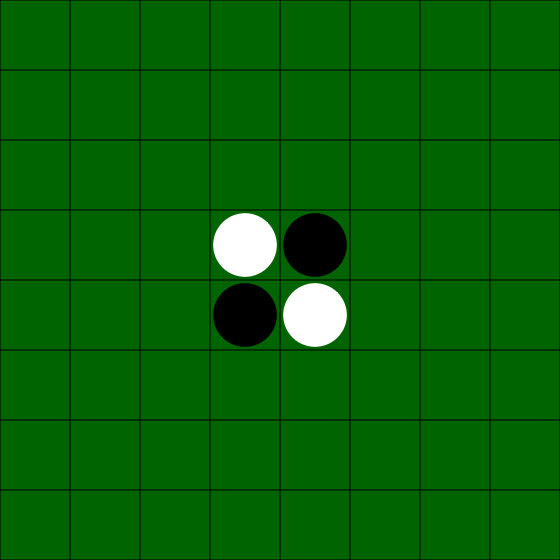
\includegraphics[width=\textwidth / 2]{board_initial}
    \caption{Initialer Spielzustand}
    \label{fig:board_initial}
\end{figure}

Zu Beginn des Spiels werden jeweils zwei Steine jedes Spielers so auf die vier mittleren Felder des Spielfelds gelegt, dass
– wie in Abbildung \ref{fig:board_initial} zu sehen – die Steine eines Spielers einander diagonal gegenüber liegen.

Die Spieler legen nun abwechselnd jeweils einen Stein ihrer eigenen Farbe auf das Spielfeld. Steine können nur auf freie
Felder gelegt werden, die in horizontale, vertikale oder diagonale Richtung an einen oder mehrere gegnerische Steine,
gefolgt von einem eigenen Stein, angrenzen. Eine beispielhafte Spielsituation, in der die möglichen Spielzüge für den
schwarzen Spieler als kleinere Kreise dargestellt werden, ist in \autoref{fig:board_possible_moves} zu sehen. 

\begin{figure}[H]
    \centering
    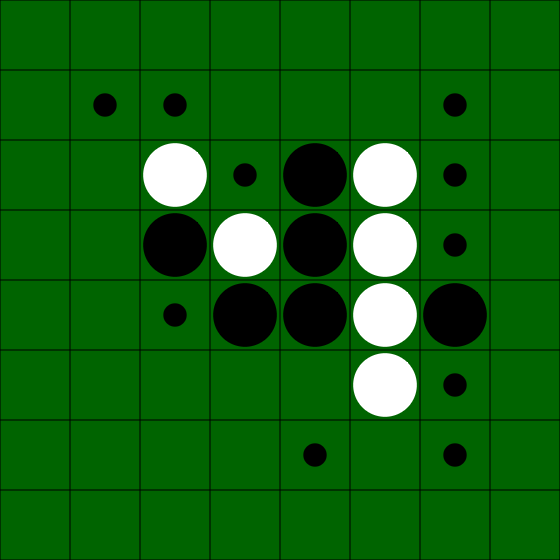
\includegraphics[width=\textwidth / 2]{board_possible_moves}
    \caption{Mögliche Züge des schwarzen Spielers}
    \label{fig:board_possible_moves}
\end{figure}

Alle gegnerischen Steine, die durch den gesetzten Stein in eine der 8 Richtungen lückenlos eingeschlossen werden, ohne dass sich freie Felder dazwischen befinden, werden umgedreht und erhalten dadurch die Farbe des Spielers, der diesen Zug ausgeführt hat.

Ist einer der Spieler zugunfähig, das heißt, er ist an der Reihe, kann jedoch keinen validen Zug spielen, so ist der
andere Spieler erneut am Zug.

Das Spiel endet, sobald beide Spieler zugunfähig sind. Der Gewinner ist dann der Spieler, der die meisten Steine seiner
Farbe auf dem Spielfeld liegen hat.
\cite{worldothellorules}


\section{Spieltheorie}
\label{sec:spieltheorie}

Eine mathematische Betrachtung von Spielen erfordert eine abstrakte Darstellung derselben. Ein Spiel kann dabei
verschiedene Eigenschaften haben. Auf das Spiel Othello treffen beispielsweise die folgenden Eigenschaften zu:

\begin{itemize}
    \item Determinismus
    \item Rundenbasiertheit
    \item Zwei-Spieler
    \item Nullsummenspiel
    \item Perfekte Information
\end{itemize}

Die Eigenschaft des Determinismus schließt auf Zufall basierende Elemente aus, die beispielsweise in Würfelspielen durch
das Würfeln einer zufälligen Zahl auftreten. Da in Othello jeder Spielzug nur von der Entscheidung des Spielers abhängt,
wird diese Eigenschaft erfüllt. Im Spielverlauf sind zudem immer zwei Spieler abwechselnd am Zug. Folglich werden auch
die Eigenschaften Zwei-Spieler und Rundenbasiertheit erfüllt. Bei einem Nullsummenspiel handelt es sich um ein
Spiel, bei dem das Ergebnis beider Spieler am Ende jedes Spiels die gleiche Summe hat. Beim Schach bekommt z. B. der
Gewinner einen Punkt und der Verlierer keinen Punkt, bei einem Unentschieden bekommen beide Spieler einen halben Punkt.
Die Summe beträgt also immer eins. Diese Regel kann auch in Othello angewandt werden, da ein Spiel entweder mit einem
Sieg und einer Niederlage oder einem Unentschieden endet. Um die Höhe des Sieges zu berücksichtigen, kann für jeden
Spieler die Anzahl der Steine gezählt werden. Dabei müssen lediglich nicht belegte Felder berücksichtigt und
beispielsweise für den Gewinner mit mehr Steinen gezählt werden. Da sich die Anzahl der Gesamtfelder nicht ändert,
beträgt die Summe der Punkte beider Spieler bei einer Spielfeldgröße von $8\times 8$ immer 64 und somit handelt es sich
bei Othello um ein Nullsummenspiel. Bei einem Spiel mit perfekter Information können beide Spieler zu jeder Zeit den
kompletten Zustand des Spiels einsehen. Anders als bei vielen Kartenspielen, in denen die Karten der
Gegenspieler unbekannt sind, ist das in Othello der Fall.
\cite[S.~161f.]{ai2010russel}

Formal besteht ein Spiel aus folgenden sechs Elementen:
\begin{enumerate}
    \item $S_0$ ist der Anfangszustand zu Beginn des Spiels.
    \item $Player(s)$ ist eine Funktion, die in einem Spielzustand $s$ den Spieler berechnet, der gerade an der Reihe
    ist.
    \item $Actions(s)$ ist eine Funktion, die für einen Spielzustand $s$ alle gültigen Züge berechnet.
    \item $Result(s, a)$ ist eine Funktion, die für einen Spielzustand $s$ und eine Aktion, also einen Spielzug $a$
    einen neuen Spielzustand berechnet.
    \item $TerminalTest(s)$ ist eine Funktion, die für einen Spielzustand $s$ berechnet, ob das Spiel vorbei ist oder
    nicht. Zustände, an denen das Spiel vorbei ist, werden Endzustände genannt.
    \item $Utility(s, p)$ ist eine Funktion, die für einen Endzustand $s$ ein numerisches Endergebnis für den Spieler
    $p$ berechnet.
\end{enumerate}


\section{Suchbäume}
\label{sec:gametree}

Ein Spiel kann als Baum dargestellt werden, dessen Wurzel gleich dem Startzustand des Spiels ist. Die Kanten des Baums
stellen Aktionen dar, die zu einem neuen Knoten, also einem neuen Spielzustand, führen. Vorerst sei angenommen, dass ein
bestimmter Spielzustand, in dem das Spiel gewonnen ist, gesucht wird und die Spielzüge des Gegners ausgesucht werden
können. Dieses Suchproblem hat als Lösung eine Abfolge von Aktionen, die zum Sieg des Spiels führen. Jeder Knoten kann
so erweitert werden, dass für jeden möglichen Spielzug, also jede Aktion, eine Kante zu einem neuen Knoten, also zu
einem neuen Spielzustand, führt. Der Baum kann dann nach einem bestimmten Zustand durchsucht werden, der das gegebene
Problem löst. Die Vorgehensweise dabei ist eine Tiefensuche. Zunächst wird eine Option bis zum Ende des Spiels
untersucht und erst wenn diese nicht zu einer Lösung des Problems führt, werden die übrigen Optionen in Betracht
gezogen.
\cite[S.~75]{ai2010russel}

\subsection{Adversative Suche}
In einem Spiel können die Züge des Gegners nicht beeinflusst werden. Deswegen ist ein einzelner Pfad von Aktionen
uninteressant und eine sogenannte Strategie, die für jeden Zug alle möglichen Reaktionen des Gegners betrachtet, ist
gesucht. Eine optimale Strategie führt unter der Annahme, dass auch der Gegner optimal spielt, zu einem mindestens
genauso guten Ergebnis wie jede andere Strategie.
\cite[S.~163f.]{ai2010russel}

Der Baum eines gesamten Spiels kann je nach Spiel sehr groß sein. Für das Spiel Othello besteht der Baum bei der Annahme
von einer durchschnittlichen Spiellänge von 58 Zügen und zehn Möglichkeiten pro Spielzug aus $10^{58}$ Knoten. Bei drei
verschiedenen Zuständen, die jedes Feld annehmen kann (frei, belegt von schwarz oder belegt von weiß), liegt die
Speicherkomplexität bei $3^{64}\approx10^{30}$ möglichen Spielzuständen. Diese Zahl lässt sich durch Ausschließen
offensichtlich ungültiger Zustände, in denen beispielsweise die mittleren vier Felder nicht belegt sind oder gesetzte
Steine nicht verbunden sind, auf ca. $10^{28}$ reduzieren \cite[S.~167]{searchingforsolutions}.
Bei einer Repräsentation von 2 Bit pro Feld, also 16 Byte pro Spielzustand, würden diese Zustände ca. $10^{20}$\,GB
Speicher benötigen. Der Spielbaum muss in diesem Fall also als theoretisches Konstrukt betrachtet werden, da er nicht
komplett dargestellt werden kann. Ein Suchbaum ist ein Teil des Spielbaums, der jedoch nur die für eine Entscheidung
relevanten Knoten beinhaltet.
\cite[S.~162f.]{ai2010russel}

Im allgemeinen Fall können Zustände mehrfach im Baum auftreten. Das passiert, wenn Spielzüge rückgängig gemacht werden
können. Beispielsweise können im Schach manche Figuren auf das vorherige Feld zurückgestellt werden. Für diese Spiele
ist es sinnvoll, zyklische Pfade auszuschließen. Dadurch wird verhindert, dass durch beliebig viele Wiederholungen eine
unendliche Menge an Pfaden entsteht.
\cite[S.~75]{ai2010russel}

In dem Spiel Othello kann allerdings kein Zustand mehrfach auftreten, da nach jedem Spielzug genau ein Spielstein mehr
auf dem Feld liegt und Spielsteine nicht wieder weggenommen werden können.


\section{Der Minimax-Algorithmus}

Minimax ist ein Algorithmus zur Bestimmung des optimalen Spielzugs in einem deterministischen, rundenbasierten, zwei-Spieler Nullsummenspiel mit perfekter Information.

Dabei wird für jeden Knoten im Spielbaum des Spiels, durch Rekursion, der Nutzen des entsprechenden Spielzustands für alle Spieler bestimmt.
An den Blatt-Knoten des Spielbaums ist der Nutzen für alle Spieler, in Form des Spielergebnisses, bereits bekannt.
Die Nutzen-Werte der restlichen Knoten werden bestimmt, indem, unter der Annahme das beide Spieler optimal spielen, immer der größte Nutzen aus den Kind-Knoten für den aktuell spielenden Spieler ausgewählt wird.
\cite[S.~165]{ai2010russel}

Dadurch lässt sich zu jedem Spielzustand der Zug bestimmen, der gegen einen optimal spielenden Gegner von größtem Nutzen ist.

Da bei einem zwei-Spieler Nullsummenspiel die Summe der Nutzen der beiden Spieler konstant ist, und sich somit der Nutzen für einem Spieler aus dem Nutzen des anderen Spielers ergibt, muss nur der Nutzen für einen Spieler betrachtet werden. Dieser wird dann abwechselnd von diesem Spieler maximiert, und von dessen Gegner minimiert.
Die Spieler werden dann maximierender und einen minimierender Spieler genannt.
Aus diesem Vorgehensweise ergibt sich der Name "'Minimax"' für die zwei-Spieler Variante des Algorithmus.
Bei Spielen mit mehr als zwei Spielern kann diese Optimierung nicht angewandt werden, weshalb in diesem Fall immer der Nutzen für alle Spieler getrennt betrachtet werden muss.
\cite[S.~165]{ai2010russel}

%TODO: Mathematische Beschreibung / evtl. Implementation





\section{Heuristische Evaluations-Funktion}

In vielen relevanten Spielen ist es aufgrund der Größe des Suchbaums praktisch nicht möglich diesen vollständing zu
durchsuchen. In der Praxis kann der Suchbaum deshalb nur bis zu einer begrenzten Tiefe durchsucht werden. An diesem
Punkt kommt eine heuristische Evaluations-Funktion zum Einsatz, welche den Nutzen des Spielzustands für einen Spieler
approximiert.
\cite[S.~171]{ai2010russel}

Optimalerweise würde die Evaluations-Funktion den tatsächlichen Nutzen einer Spielsituation bestimmen. Eine solche
Evaluations-Funktion ist durch den Minimax Algorithmus gegeben. Aus offensichtlichen Gründen, kann diese jedoch nicht
zum Einsatz kommen, da der Rechenaufwand hierbei identisch zu einer vollständigen Suche wäre.

Um den Nutzen verschiedener Spielzüge miteinander zu vergleichen, wird also eine weniger rechenaufwändige
Evaluations-Funktion benötigt, die diesen nur ausreichend gut annähert, statt den tatsächlichen Nutzen zu bestimmen.

Durch die Anwendung einer approximierten Evaluations-Funktion verliert der Minimax Algorithmus seine Optimalität. Es
wird also nichtmehr garantiert der Zug mit dem größten Nutzen gewählt. Mit einer passend gewählten Evaluations-Funkion
können dennoch gute Ergebnisse erzielt werden, die in vielen Spielen die Fähigkeiten eines menschlichen Gegenspielers
übertreffen. Die Spielstärke der KI wächst mit zunehmender Suchtiefe.

Ein primitiver Ansatz für eine Evaluations-Funktion bei dem Spiel Othello ist die Differenz der Anzahlen von eigenen
Steinen und gegnerischen Steinen auf dem Spielfeld, da diese am Ende über den Sieg entscheidet. Gegen Ende eines Spiels
könnte dieser Ansatz eine passende Bewertung liefern, allerdings kann es vor allem in der Anfangsphase sinnvoll sein,
weniger Steine zu haben. Viel wichtiger ist z.\,B. die Möglichkeit, neue Steine zu platzieren.

Diesen Ansatz verfolgt die Betrachtung der Mobilität.

Die aktuelle Mobilität ist ein Maß dafür, wie viele mögliche Züge die Spieler haben. Eine niedrige Anzahl an möglichen
Zügen ist häufig schlecht, da der Spieler gezwungen ist, einen weniger guten Zug zu machen. Als quantitatives Merkmal
kann zunächst die Differenz der möglichen Züge beider Spieler betrachtet werden. Allerdings ist eine Stellung häufig
besser, wenn man mehr mögliche Züge hat und der Gegner bei gleicher Differenz weniger mögliche Züge hat. Um diese
Tatsache zu berücksichtigen, kann eine nicht-lineare Funktion verwendet werden.
%TODO: Buro verwendet aus Performancegründen eine Approximation
\cite[S. 7]{evaluationfunctions}

Neben der aktuellen Mobilität kann auch die potenzielle Mobilität betrachtet werden. Diese ist ein Indikator für die
mögliche Mobilität in folgenden Zügen. Michael Buro hat als aussagekräftigstes Merkmal die Summe aller Anzahlen freier
Felder um gegnerische Steine ausgemacht.
\cite[S. 8f.]{evaluationfunctions}


\section{Alpha-Beta-Pruning}

Die Alpha-Beta-Pruning ist eine Optimierung des Minimax Algorithmus, bei der komplette Zweige des Suchbaums ausgeschlossen werden können, die das Ergebnis des Algorithmus' nicht mehr beeinflussen können.
Ein Zweig kann ausgeschlossen werden, wenn für einen Spieler bereits ein Zug mit einem größeren Nutzen gefunden wurde, als bei dem zu betrachtenden Zweig maximal noch erzielbar ist.

Durch Anwendung von Alpha-Beta-Pruning wird das Ergenis des Minimax Algorithmus' nicht beeinflusst. Jeoch kann durch die Betrachtung einer geringeren Zahl von Knoten die Performanz signifikant verbessert werden.

Bei einer nicht vollständingen Alpha-Beta-Suche, unter Anwendung einer heuristischen Evaluations-Funktion kann gegenüber dem Minimax Algorithmus die maximale Suchtiefe bei gleicher Rechenzeit erhöht werden, was zu einem besseren Ergebnis führt.

Da Alpha-Beta-Pruning nur dann Zweige ausschließen kann, wenn bereits bessere Zweige betrachtet wurden ist es von Vorteil, die Zweige in der Reihenfolge absteigenden Nutzens zu betrachten, da so die Anzahl der ausgeschlossenen
Zweige maximiert werden kann.
Dies ist jedoch in der Praxis nicht optimal möglich, da dafür ja bereits eine korrekte Bewertung der Züge stattgefunden haben muss, was die Anwendung der Alpha-Beta Suche überflüssig machet.
Eine ungefähre Anordnung der Züge, die dennoch zu einer wesentlichen Effizienzverbesserung führt ist jedoch häufig möglich. Beispielsweise können beim Schach Züge in denen eine gegnerische Figur
geschlagen wird priorisiert werden, und beim Othello Züge in den Ecken und am Rand des Spielfelds, gegenüber denen in der Mitte bevorzugt werden.

\section{ProbCut}

Der Minimax-Algorithmus erfordert in seiner Grundform das Durchsuchen des kompletten Spielbaums.
Die Optimierung des Alorithmus durch die Alpha-Beta-Suche ermöglicht zwar das Weglassen von Teilen des Spielbaums, aber da auch hier der korrekte Minimax-Wert berechnet werden muss, kann der Baum nur rückwärts reduziert werden.

ProbCut erweitert die Alpha-Beta-Suche durch eine statistische Betrachtung, wobei auch Zweige, die nur mit einer bestimmten Wahrscheinlichkeit nicht zu einer Veränderung des Ergebnisses beitragen, weggelassen werden können.
Die mithilfe von ProbCut durchgeführten Verkleinerungen des Baums werden "`probabilistic forward cuts"' genannt.

Ein Zug ist dann für die Entscheidung irrelevant, wenn dessen Minimax Wert außerhalb des Alpha-Beta Fensters, dh. außerhalb des Intervalls \([\alpha,\beta]\) liegt, da dieser Zug von beiden Spielern umgangen wird und deshalb im Spiel nicht auftritt.
Dies entspricht der Abbruchbedingung beim Alpha-Beta Algorithmus.
Ob das der Fall ist ist jedoch in der Regel erst nach Anwendung des Alpha-Beta Algorithmus' mit der maximal gewünschten Suchtiefe bekannt.

ProbCut stellt einen statistischen Zusammenhang zwischen dem Minimax Wert einer tieferen Suche der Tiefe \(d\) und dem Wert einer flacheren Suche der Tiefe \(d'<d\) her.
Anhand des Minimax Werts der flachen Suche wird bestimmt ob der Wert der tiefen Suche mit einer gegebenen Wahrscheinlichkeit \(p\) außerhalb des Alpha-Beta Fensters liegt.
Ist dies der Fall so wird bereits nach der flachen Suche abgebrochen, sodass die Tiefe Suche nicht mehr durchgeführt werden muss.

Dazu verwendet ProbCut ein lineares statistisches Modell \(v=a*v'+b+e\) wobei \(v\) der Minimax Wert der tiefen Suche, \(v'\) der Minimax Wert der flachen Suche, \(a\) und \(b\) konstanten und \(e\) eine normalverteilte Fehlervariable ist.
\(a\) und \(b\) werden im Vorraus so gewählt dass die Standardabweichung \(\sigma\) von \(e\) möglichst gering ist.

Daraus lässt sich herleiten dass mit einer Wahrscheinlichkeit von mindestens \(p\) gilt:

\(v<=\alpha\) genau dann wenn \(v'<=(\Phi^{-1}(p)*\sigma+\alpha-b)/a\)

und

\(v>=\beta\) genau dann wenn \(v'>=(-\Phi^{-1}(p)*\sigma+\beta-b)/a\)

Trifft nach der flachen Suche einer der beiden Fälle auf der rechten Seite ein, so wird keine tiefe Suche durchgeführt, da \(v\) nach der linken Seite min Wahrscheinlichkeit \(p\) ausßerhalb des Alpha-Beta Fensters liegt
und somit nicht relevant ist.

Wie auch beim Alpha-Beta Algorithmus ergibt sich der Vorteil von ProbCut durch die Zeitersparnis, die durch das Weglassen von Zweigen erreicht wird. Dadurch kann die Suchtiefe bei den relevanten Zweigen erhöht werden.
\cite[S.~1]{probcut}


	%!TEX root = ../dokumentation.tex

\chapter{Implementation}
\label{chap:implementation}

Dieses Kapitel befasst sich mit der Implementation der Künstlichen Intelligenz. Dazu gehört zunächst die Implementation
der Spiellogik von Othello, die Implementation der eigentlichen Künstlichen Intelligenz unter Anwendung der im
\autoref{chap:theorie} genannten Techniken, außerdem mehrere Experimente zur Bestimmung der optimalen Parameter, sowie eine Grafische
Benutzeroberfläche zum Testen der Künstlichen Intelligenz. Die Implementation dieser Komponenten erfolgt in der
Programmiersprache Python unter Verwendung von Jupyter Notebooks. 

\hypertarget{spiellogik-othello_game.ipynb}{%
\section{Spiellogik
(othello\_game.ipynb)}\label{spiellogik-othello_game.ipynb}}

\label{sec:gamelogic} \ifx false

\begin{lstlisting}[language=Python]
%%HTML
<style>
.container { width:100% }
</style>
\end{lstlisting}

\fi Im Folgenden ist die Spielelogik des Spiels Othello implementiert.
Dazu gehört die Implementierung aller im \autoref{sec:spieltheorie}
genannten Aspekte, wie zum Beispiel die Erzeugung eines Startzustands,
sowie die Bestimmung und Durchführung von Spielzügen ausgehend von einem
Spielzustand.

\hypertarget{importieren-der-externen-abhuxe4ngigkeiten}{%
\subsection{Importieren der externen
Abhängigkeiten}\label{importieren-der-externen-abhuxe4ngigkeiten}}

Die Implementierung stützt sich für bessere Performanz auf die
Python-Bibliothek \passthrough{\lstinline!numpy!}, welche unter anderem
homogene Felder und Matrizen implementiert. Eine solche Matrix wird als
interne Repräsentation des Othello Spielfelds genutzt. Insbesondere
Operationen, die auf einen größeren Teil des Spielfelds zugreifen
müssen, können dadurch beschleunigt werden.

Für das Kopieren der Spielzustände wird das Modul
\passthrough{\lstinline!copy!} aus der Python Standardbibliothek
verwendet.

\begin{lstlisting}[language=Python]
import numpy as np
import copy
\end{lstlisting}

\hypertarget{globale-konstanten}{%
\subsection{Globale Konstanten}\label{globale-konstanten}}

Im folgenden Abschnitt werden zunächst einige Konstanten definiert,
welche in der späteren Implementierung häufig genutzt werden.

Die Konstante \passthrough{\lstinline!BOARD\_SIZE!} gibt die Anzahl an
Zeilen und Spalten des quadratischen Othello Spielfelds an.
\passthrough{\lstinline!BOARD\_SIZE!} wird beispielsweise zur Iteration
über Zeilen und Spalten des Spielfeldes genutzt, sowie zur Überprüfung,
ob gegebene Koordinaten innerhalb des Spielfeldes liegen.

Die Konstanten \passthrough{\lstinline!BLACK!},
\passthrough{\lstinline!WHITE!} und \passthrough{\lstinline!NONE!}
werden auf die Zahlenwerte -1, 1 und 0 abgebildet und werden für mehrere
Zwecke genutzt:

\begin{enumerate}
\def\labelenumi{\arabic{enumi}.}
\tightlist
\item
  Repräsentation des Spielfeldes: Das Othello Spielbrett wird als
  \(8\times 8\) Matrix von Ganzzahlen definiert, welche jeweils einen
  der drei Werte annehmen können. Hierbei stehen die Werte
  \passthrough{\lstinline!BLACK!} und \passthrough{\lstinline!WHITE!}
  jeweils für einen Stein des jeweiligen Spielers, während
  \passthrough{\lstinline!NONE!} ein leeres Feld repräsentiert.
\item
  Repräsentation der Spieler: \passthrough{\lstinline!BLACK!} und
  \passthrough{\lstinline!WHITE!} werden zur Repräsentation eines
  Spielers genutzt. Beispielsweise enthält der Spielzustand eine
  Variable \passthrough{\lstinline!turn!}, die angibt, welcher Spieler
  am Zug ist.
\item
  Berechnung der Heuristiken: Die Werte \passthrough{\lstinline!BLACK!},
  \passthrough{\lstinline!WHITE!} und \passthrough{\lstinline!NONE!}
  sind so gewählt, dass sie sich für die Berechnung der Heuristiken
  eignen. Der in der \ac{KI} maximierende Spieler hat den positiven Wert
  1, während der minimierende Spieler durch den negativen Wert -1
  repräsentiert wird. Kein Spieler wird durch den Wert 0 dargestellt.
\end{enumerate}

\begin{lstlisting}[language=Python]
BOARD_SIZE = 8

BLACK = -1  # MINIMIZING PLAYER
WHITE =  1  # MAXIMIZING PLAYER
NONE  =  0  # NO PLAYER
\end{lstlisting}

\hypertarget{game-state}{%
\subsection{Game State}\label{game-state}}

Die Klasse \passthrough{\lstinline!GameState!} repäsentiert einen
Spielzustand von Othello. Dieser wird durch die im Folgenden genannten
Attribute beschrieben:

\begin{itemize}
\tightlist
\item
  Das Spielfeld \passthrough{\lstinline!board!}, welches durch eine
  zweidimensionale Numpy-Matrix repräsentiert wird, bei der jede Zelle
  die die Werte \passthrough{\lstinline!BLACK!},
  \passthrough{\lstinline!WHITE!} und \passthrough{\lstinline!NONE!}
  annehmen kann.
\item
  Den Spieler \passthrough{\lstinline!turn!}, der im Spielzustand am Zug
  ist. Zusätzlich enthält der Spielzustand weitere Informationen, die
  zur Verbesserung der Performanz genutzt werden.
\item
  Die im aktuellen Spielzustand möglichen Züge werden als Paare von
  Koordinaten in der Variable \passthrough{\lstinline!possible\_moves!}
  gespeichert. Ein Koordinatenpaar steht hierbei für das Setzen eines
  Spielsteins auf die entsprechende Stelle auf dem Spielfeld unter
  Anwendung der Othello Regeln. Diese Variable ist Teil von
  \passthrough{\lstinline!GameState!}, damit pro Spielzustand die
  möglichen Züge nicht mehrfach berechnet werden müssen.
\item
  Die Menge der freien Felder, die horizontal, vertikal oder diagonal an
  einen Stein angrenzen wird in der Variable
  \passthrough{\lstinline!frontier!} gespeichert. Beim Ermitteln der
  möglichen Züge kann dadurch die Performanz wesentlich gesteigert
  werden, da nur diese Menge und nicht das gesamte Spielfeld überprüft
  werden muss.
\item
  Die Anzahl an Spielsteinen auf dem Spielfeld wird in der Variable
  \passthrough{\lstinline!num\_pieces!} gehalten.
\item
  Ob der Spielzustand ein Endzustand ist, wird in der Variable
  \passthrough{\lstinline!game\_over!} gespeichert.
\item
  Die Koordinaten des letzten Spielzugs werden zur späteren
  Visualisierung in der \ac{GUI} in der Variable
  \passthrough{\lstinline!last\_move!} gespeichert.
\end{itemize}

Die zur Performance-Verbesserung genutzten Variablen werden im Laufe des
Spielverlaufs immer aktuell gehalten.

In dem Konstruktor \passthrough{\lstinline!\_\_init\_\_!} der Klasse
\passthrough{\lstinline!GameState!} wird ein neuer Spielzustand
entsprechend den Othello Spielregeln instanziiert, indem alle Variablen
entsprechend initialisiert werden.

Die Funktion \passthrough{\lstinline!\_\_lt\_\_!} ist implementiert,
damit auf \passthrough{\lstinline!GameState!}-Objekten der
Vergleichsoperator angewendet werden kann. Das ist nötig, damit in der
\ac{KI} Tupel sortiert werden können, die beispielsweise aus einer
Priorität und einen \passthrough{\lstinline!GameState!} bestehen. Da in
diesem Fall nur die Sortierung nach der Priorität wichtig ist, ist die
Implementierung von \passthrough{\lstinline!\_\_lt\_\_!} irrelevant.
Daher wird der Einfachkeit halber immer True zurückgegeben.

\begin{lstlisting}[language=Python]
class GameState:
    def __init__(self):
        self.board = np.zeros((BOARD_SIZE, BOARD_SIZE), dtype=np.int8)
        self.board[3, 3] = WHITE
        self.board[3, 4] = BLACK
        self.board[4, 3] = BLACK
        self.board[4, 4] = WHITE
        self.turn = BLACK
        self.possible_moves = [(2, 3), (3, 2), (4, 5), (5, 4)]
        self.frontier = {(2, 2), (2, 3), (2, 4), (2, 5),
                         (3, 2), (3, 5), (4, 2), (4, 5),
                         (5, 2), (5, 3), (5, 4), (5, 5)}
        self.num_pieces = 4
        self.game_over = False
        self.last_move = None

    def __lt__(self, other):
        return True
\end{lstlisting}

Die Liste \passthrough{\lstinline!directions!} enthält alle
horizontalen, vertikalen und diagonalen Richtungen auf dem Spielfeld als
Zwei-Tupel. Die beiden Zahlen stellen hierbei jeweils den Versatz in
Reihen- und Spaltenrichtung dar. Diese Liste wird später in mehreren
Funktionen genutzt.

\begin{lstlisting}[language=Python]
directions = [(-1,-1),(0,-1),(1,-1),(-1,0),(1,0),(-1,1),(0,1),(1,1)]
\end{lstlisting}

Die Exception \passthrough{\lstinline!InvalidMoveException!}, wird
später in der Funktion \passthrough{\lstinline!make\_move!} geworfen,
wenn ein ungültiger Spielzug gefordert wird. Dies dient der
Fehlerbehandlung.

\begin{lstlisting}[language=Python]
class InvalidMoveException(Exception):
    pass
\end{lstlisting}

Die Funktion \passthrough{\lstinline!can\_flip\_in\_dir!} überprüft für
ein Spielfeld \passthrough{\lstinline!board!} und den Spieler
\passthrough{\lstinline!player!}, ob beim Setzen eines Steins auf die
Position \passthrough{\lstinline!pos!} in die Richtung
\passthrough{\lstinline!direction!} nach den Regeln von Othello Steine
umgedreht werden können. Die Variable \passthrough{\lstinline!board!}
enthält das Spielfeld als Python-Liste, da einzelne Zugriffe so deutlich
schneller sind, als bei einem Numpy-Array.
\passthrough{\lstinline!can\_flip\_in\_dir!} gibt einen Wahrheitswert
zurück. Dabei bedeutet \passthrough{\lstinline!True!}, dass Steine
umgedreht werden können.

\begin{lstlisting}[language=Python]
def can_flip_in_dir(board, pos, direction, player):
    row, col = pos
    rowdelta, coldelta = direction
    current_row = row + rowdelta
    current_col = col + coldelta
    if not (0 <= current_row < 8 and 0 <= current_col < 8):
        return False
    if not board[current_row][current_col] == -player:
        return False
    current_row += rowdelta
    current_col += coldelta
    
    while True:
        if not (0 <= current_row < 8 and 0 <= current_col < 8):
            return False
        if board[current_row][current_col] == NONE:
            return False           
        if board[current_row][current_col] == player:
            return True
    
        current_row += rowdelta
        current_col += coldelta
\end{lstlisting}

Die Funktion \passthrough{\lstinline!is\_move\_valid!} überprüft für ein
gegebenes Spielfeld \passthrough{\lstinline!board!}, ob ein Zug auf die
Position \passthrough{\lstinline!pos!} für den Spieler
\passthrough{\lstinline!player!} möglich ist. Das Ergebnis wird als
Wahrheitswert zurückgegeben. \passthrough{\lstinline!board!} ist hier
ebenfalls eine Python-Liste, da der Zugriff auf einzelne Elemente
schneller ist, als bei einem Numpy-Array.

\begin{lstlisting}[language=Python]
def is_move_valid(board, pos, player):
    for direction in directions:
        if can_flip_in_dir(board, pos, direction, player):
            return True
    return False
\end{lstlisting}

\passthrough{\lstinline!get\_utility!} bestimmt für einen
Endspielzustand \passthrough{\lstinline!state!} den Gewinner des Spiels
anhand der Anzahl an Spielsteinen, die beide Spieler auf dem Spielfeld
haben. Gewinnt Weiß, so wird der Wert der Konstante
\passthrough{\lstinline!WHITE!} zurückgegeben. Gewinnt Schwarz, wird der
Wert der Konstante \passthrough{\lstinline!BLACK!} zurückgegeben. Bei
einem Unentschieden wird der Wert von \passthrough{\lstinline!NONE!}
zurückgegeben.

\begin{lstlisting}[language=Python]
def get_utility(state):
    black_disks = count_disks(state, BLACK)
    white_disks = count_disks(state, WHITE)
    if black_disks > white_disks:
        return BLACK
    if white_disks > black_disks:
        return WHITE
    else:
        return NONE
\end{lstlisting}

Die Funktion \passthrough{\lstinline!get\_possible\_moves!} bestimmt für
einen Spielzustand \passthrough{\lstinline!state!} und den Spieler
\passthrough{\lstinline!player!} alle möglichen Züge, die
\passthrough{\lstinline!player!} im Spielzustand
\passthrough{\lstinline!state!} machen kann. Die resultierenden Züge
werden als Liste von Koordinatenpaaren zurückgegeben. Für eine bessere
Performanz werden nur Felder aus der Menge
\passthrough{\lstinline!frontier!} als mögliche Züge betrachtet.

\begin{lstlisting}[language=Python]
def get_possible_moves(state, player):
    board = state.board.tolist()
    possible_moves = []
    for pos in state.frontier:
        if is_move_valid(board, pos, player):
            possible_moves.append(pos)
    return possible_moves
\end{lstlisting}

Die Funktion \passthrough{\lstinline!flip\_in\_dir!} dreht im
Spielzustand \passthrough{\lstinline!state!}, ausgehend von dem durch
\passthrough{\lstinline!pos!} angegebenen Feld, die für den Spieler
\passthrough{\lstinline!player!} gegnerischen Steine in die Richtung
\passthrough{\lstinline!direction!} um. Der eingegebene
\passthrough{\lstinline!state!} wird dabei modifiziert. Die Funktion hat
keinen Rückgabewert.

\begin{lstlisting}[language=Python]
def flip_in_dir(state, pos, direction, player):
    (row, col) = pos
    rowdelta, coldelta = direction
    current_row = row + rowdelta
    current_col = col + coldelta
    
    while state.board[current_row, current_col] == -player:
        state.board[(current_row, current_col)] = player
        current_row += rowdelta
        current_col += coldelta
\end{lstlisting}

\passthrough{\lstinline!update\_frontier!} wird nach jedem Zug
aufgerufen, um die Menge \passthrough{\lstinline!frontier!} des
Spielzustands \passthrough{\lstinline!state!} zu aktualisieren. Die
durch \passthrough{\lstinline!pos!} gegebene Koordinate wird entfernt,
während die Koordinaten aller leeren umliegenden Felder hinzugefügt
werden. Der Spielzustand \passthrough{\lstinline!state!} wird hierbei
direkt verändert und es wird kein Wert zurückgegeben.

\begin{lstlisting}[language=Python]
def update_frontier(state, pos):
    (row, col) = pos
    for current_row in range(row-1, row+2):
        if not 0 <= current_row < 8:
            continue
        for current_col in range(col-1, col+2):
            if not 0 <= current_col < 8:
                continue
            if state.board[current_row, current_col] == NONE:
                state.frontier.add((current_row, current_col))
    state.frontier.remove((row, col))
\end{lstlisting}

Die Funktion \passthrough{\lstinline!count\_disks!} zählt die Steine,
die der Spieler \passthrough{\lstinline!player!} im Spielzustand
\passthrough{\lstinline!state!} auf dem Spielfeld hat. Die resultierende
Anzahl wird von der Funktion zurückgegeben.

\begin{lstlisting}[language=Python]
def count_disks(state, player):
    return np.count_nonzero(state.board == player)
\end{lstlisting}

\passthrough{\lstinline!get\_player\_string!} konvertiert die
Zahlenrepräsentation des Spielers \passthrough{\lstinline!player!} in
den Namen des Spielers. Ist \passthrough{\lstinline!player == NONE!}, so
wird `Nobody' zurückgegeben.

\begin{lstlisting}[language=Python]
def get_player_string(player):
    return {BLACK: 'Black', WHITE: 'White', NONE: 'Nobody'}[player]
\end{lstlisting}

Die Funktion \passthrough{\lstinline!make\_move!} versucht auf einem
Spielzustand \passthrough{\lstinline!state!} einen Spielzug entsprechend
den Othello Regeln auszuführen. Der auszuführende Zug wird hierbei durch
den Parameter \passthrough{\lstinline!pos!} bestimmt, welcher die
Spielfeldkoordinaten des zu setzenden Steins als Zwei-Tupel angibt.

Zunächst wird überprüft, ob die Koordinate \passthrough{\lstinline!pos!}
in der Variable \passthrough{\lstinline!frontier!} enthalten ist. Ist
dies nicht der Fall, so kann die Funktion mit einer
\passthrough{\lstinline!InvalidMoveException!} abgebrochen werden, da
ein Spielstein nur auf ein leeres Feld gesetzt werden kann, welches an
einen Spielstein angrenzt. Hierbei handelt es sich um eine Maßnahme zur
Performanceoptimierung.

Ist \passthrough{\lstinline!pos!} in \passthrough{\lstinline!frontier!},
so wird der Spielzustand kopiert, um den ursprünglich übergebenen
Spielzustand nicht zu verändern.

Anschließend werden alle gegnerischen Steine umgedreht, welche vom neu
gesetzten Stein eingeschlossen werden. Wenn mindestens ein Stein
umgedreht wurde, wird \passthrough{\lstinline!disks\_flipped!} auf
\passthrough{\lstinline!True!} gesetzt. Wenn das nicht der Fall war,
handelt es sich nicht um einen gültigen Zug und es wird eine
\passthrough{\lstinline!InvalidMoveException!} geworfen. Andernfalls
wird der neue Stein gesetzt und im resultierenden Zustand die Variablen
\passthrough{\lstinline!frontier!}, \passthrough{\lstinline!turn!},
\passthrough{\lstinline!game\_over!} und
\passthrough{\lstinline!possible\_moves!} aktualisiert.

Der Rückgabewert der Funktion ist der neue Spielzustand.

\begin{lstlisting}[language=Python]
def make_move(state, pos):
    if pos not in state.frontier:
        print(pos, "not in Frontier")
        raise InvalidMoveException
    
    state = copy.deepcopy(state)
    disks_flipped = False
    board = state.board.tolist()
    for direction in directions:
        if can_flip_in_dir(board, pos, direction, state.turn):
            disks_flipped = True
            flip_in_dir(state, pos, direction, state.turn)

    if disks_flipped:
        state.num_pieces += 1
        state.board[pos] = state.turn
        state.last_move = pos
        update_frontier(state, pos)
        state.turn = -state.turn
        state.possible_moves = get_possible_moves(state, state.turn)
        if len(state.possible_moves) == 0:
            state.turn = -state.turn
            state.possible_moves = get_possible_moves(state, state.turn)
            if len(state.possible_moves) == 0:
                state.game_over = True
                return state
    else:
        raise InvalidMoveException()
    return state
\end{lstlisting}

Die Funktion \passthrough{\lstinline!make\_state!} erzeugt einen
Spielzustand aus einem beliebig vorbelegtem Spielfeld
\passthrough{\lstinline!board!} und dem zu ziehenden Spieler
\passthrough{\lstinline!turn!}. Diese Funktion wird zur Konstruktion von
zum Testen genutzten Spielsituationen verwendet. Der resultierende
\passthrough{\lstinline!GameState!} wird von der Funktion zurückgegeben.

\begin{lstlisting}[language=Python]
def make_state(board, turn):
    state = GameState()
    state.board = board
    state.turn = turn
    state.frontier = set()
    for row in range(8):
        for col in range(8):
            for current_row in range(row-1, row+2):
                if not 0 <= current_row < 8:
                    continue
                for current_col in range(col-1, col+2):
                    if not 0 <= current_col < 8:
                        continue
                    if state.board[current_row, current_col] == NONE:
                        state.frontier.add((current_row, current_col))
            
    state.possible_moves = get_possible_moves(state, turn)
    state.game_over = False
    if len(state.possible_moves) == 0:
        if len(get_possible_moves(state, -turn)) == 0:
            state.game_over = True
    state.num_pieces = count_disks(state, WHITE) + count_disks(state, BLACK)
    state.last_move = None
    return state
\end{lstlisting}

\hypertarget{ki-implementierung-othello_ai.ipynb}{%
\section{KI Implementierung
(othello\_ai.ipynb)}\label{ki-implementierung-othello_ai.ipynb}}

\label{sec:aiimpl} \ifx false

\begin{lstlisting}[language=Python]
%%HTML
<style>
.container { width:100% }
</style>
\end{lstlisting}

\fi

Dieses Kapitel beschreibt die Implementierung der \ac{KI}. Es werden
mehrere unterschiedliche Strategien implementiert, um einen Vergleich
von diesen zu ermöglichen.

\hypertarget{importieren-der-externen-abhuxe4ngigkeiten}{%
\subsection{Importieren der externen
Abhängigkeiten}\label{importieren-der-externen-abhuxe4ngigkeiten}}

Zur Initialisierung der Parameter \passthrough{\lstinline!alpha!} und
\passthrough{\lstinline!beta!} in der mit Alpha-Beta Pruning optimierten
Minimax Strategie werden die Konstanten
\passthrough{\lstinline!math.inf!} und
\passthrough{\lstinline!-math.inf!} benötigt. Sie stehen jeweils für den
maximalen und den minimalen Wert, den eine Fließkommazahl annehmen kann.
Die Konstanten werden von der Python Standardbibliothek in dem Modul
\passthrough{\lstinline!math!} bereitgestellt

Das Modul \passthrough{\lstinline!random!} wird im Rahmen dieser
Implementierung für mehrere Zwecke genutzt. Zum einen zur
Implementierung der \passthrough{\lstinline!random\_ai!}, einer
Strategie, welche immer einen zufälligen Zug wählt und zum anderen, um
die auf Minimax basierenden Strategien nicht-deterministisch zu machen.

\begin{lstlisting}[language=Python]
import math
import random
\end{lstlisting}

Die Implementierung der \ac{KI} baut auf der Implementierung der
Spielelogik von Othello auf. Das entsprechende Notebook muss also hier
ausgeführt werden.

\begin{lstlisting}[language=Python]
%run othello_game.ipynb
\end{lstlisting}

Die aktuellen Nutzen-Werte der beiden Spieler werden in der globalen
Variable utilities gespeichert, sodass diese in der GUI angezeigt werden
können. Diese Werte werden in den entsprechenden Funktionen der
Strategien aktualisiert.

\begin{lstlisting}[language=Python]
utilities = {WHITE: '-', BLACK: '-'}
\end{lstlisting}

\hypertarget{heuristiken}{%
\subsection{Heuristiken}\label{heuristiken}}

Zum Abschätzen der Nützlichkeit eines Spielzustands wird eine Heuristik
benötigt. Im Folgenden sind einige solcher Heuristiken implementiert. Da
Weiß der maximierende Spieler und Schwarz der minimierende Spieler ist,
repräsentiert ein höherer Wert der Heuristik einen für Weiß
vorteilhaften Zug, während ein niedriger Wert einen Vorteil für Schwarz
repräsentiert. Die Werte aller Heuristiken liegen zwischen \(-1\) und
\(1\), wobei diese Randwerte einen garantierten Sieg für den jeweiligen
Spieler darstellen. Der Wert \(0\) steht für einen für beide Spieler
gleich guten Spielzustand.

Die Funktion \passthrough{\lstinline!disc\_count\_heuristic!}
implementiert die in \ref{sec:disccount} beschriebene Heuristik. Dafür
wird die Differenz der Anzahlen an Steinen beider Spieler auf dem
Spielfeld bestimmt. Diese wird zur Normalisierung durch die maximale
Steinzahl \(64\) geteilt.

\begin{lstlisting}[language=Python]
def disc_count_heuristic(state):
    return (count_disks(state, WHITE) - count_disks(state, BLACK)) / 64
\end{lstlisting}

\passthrough{\lstinline!mobility\_heuristic!} berechnet wie in
\ref{sec:theorycurrentmobility} beschrieben die aktuelle Mobilität. Auch
dieser Wert wird durch Division durch die Anzahl an Feldern
normalisiert, um die Grenzen von \(-1\) und \(1\) einzuhalten. Zu
beachten ist hier, dass auch die Anzahl möglicher Züge für einen Spieler
bestimmt wird, der im Spielzustand gar nicht am Zug ist. Dies wirkt
zunächst sematisch nicht sinvoll, hat sich jedoch, wie in
\ref{sec:currentmobility} gezeigt, im Vergleich gegenüber möglicher
Alternativen, wie der Verwendung einer durchschnittlichen Mobilität, als
effektiver erwiesen.

\begin{lstlisting}[language=Python]
def mobility_heuristic(state):
    if state.turn == WHITE:
        return (len(state.possible_moves) -
                len(get_possible_moves(state, BLACK))) / 64
    else:
        return (len(get_possible_moves(state, WHITE)) -
                len(state.possible_moves)) / 64
\end{lstlisting}

Nicht nur die aktuelle, sondern auch die potenzielle Mobilität, welche
in \ref{sec:potmobility} beschrieben wird, kann vor allem in frühen
Phasen des Spiels wichtig für die Bewertung einer Position sein. Die
Funktion \passthrough{\lstinline!pot\_mob\_heuristic!} berechnet für
einen Zustand \passthrough{\lstinline!state!} die Differenz der
potenziellen Mobilität beider Spieler. Die potenzielle Mobilität eines
Spielers ist hierbei gegeben durch die Summe aller freier Felder um
gegnerische Spielsteine, da Michael Buro dieses Merkmal in seiner
Dissertation als beste Metrik für die potenzielle Mobilität ausgemacht
hat \cite[S. 9]{evaluationfunctions}. Das Ergebnis wird durch \(3.5\)
geteilt, da es in zufälligen Spielen im Durchschnitt \(3.5\) mal so
viele potenzielle Züge wie tatsächliche Züge gibt.

\begin{lstlisting}[language=Python]
def pot_mob_heuristic(state):
    board = list(state.board)
    fields = 0
    for (x,y) in state.frontier:
        for dx, dy in directions:
            xi = x + dx
            yi = y + dy
            if 0 <= xi < 8 and 0 <= yi < 8 and board[xi][yi] != 0:
                fields -= board[xi][yi]
    fields /= 3.5 
    return fields / 64
\end{lstlisting}

Die Funktion \passthrough{\lstinline!combined\_mobility\_heuristic!}
kombiniert die aktuelle und potenzielle Mobilität, wobei zu Beginn des
Spiels die potenzielle Mobilität stärker gewichtet wird und gegen Ende
des Spiels die aktuelle Mobilität. Michael Buro beschreibt in seiner
Dissertation, dass die potenzielle Mobilität, bis 36 Spielsteine auf dem
Feld liegen, wichtiger für die Bewertung ist, als die aktuelle Mobilität
\cite[S. 9]{evaluationfunctions}. Eigene Tests, welche in Kapitel
\ref{sec:combinedmobility} beschrieben sind, ergeben, dass eine lineare
Kombination der beiden Merkmale zu einem guten Ergebnis führt.

\begin{lstlisting}[language=Python]
def combined_mobility_heuristic(state):
    act = mobility_heuristic(state)
    pot = pot_mob_heuristic(state)
    return (1 - state.num_pieces / 50) * pot + (state.num_pieces / 50) *  act
\end{lstlisting}

Beim Spielen von Othello fällt auf, dass es bestimmte Felder gibt, deren
Belegung von Vorteil ist, sowie einige, deren Belegung eher nachteilhaft
ist. Diese Eigenschaft macht sich die Cowthello-Heuristik
\cite{cowthello} zunutze, welche in \ref{sec:cowthello} beschrieben ist.
Sie weist jedem Feld einen Wert zu, der angibt, wie vorteilhaft der
Besitz dieses Feldes ist, bzw. wie nachteilhaft die Belegung des Feldes
durch den Gegner ist. Diese Gewichte werden mit der aktuellen Belegung
des Spielfelds multipliziert und die Ergebnisse anschließend
aufsummiert. Der resultierende Wert schätzt dann den Nutzen der
aktuellen Position ein. Auch bei dieser Heuristik findet eine
Normalisierung statt.

Aufgrund der Symmetrie des Othello Spielfeldes ist es für die
Weight-Heuristik nicht nötig, für jedes Feld einzeln dessen Gewicht
anzugeben. Stattdessen werden ausschließlich die Gewichte für ein
Viertel des Spielfelds angegeben und dieses anschließend gespiegelt. Die
Funktion \passthrough{\lstinline!gen\_cowthello\_matrix!} generiert dann
die Gewichte-Matrix für das gesamte Feld und führt auch die
Normalisierung durch. Dabei werden die Gewichte aus dem Online-Othello
Programm Cowthello \cite{cowthello} verwendet. Cowthello ist unter der
URL \url{https://www.aurochs.org/games/cowthello/} verfügbar.

\begin{lstlisting}[language=Python]
def gen_cowthello_matrix():
    quarter = np.array([
        [100, -25, 25, 10],
        [-25, -50,  1,  1],
        [ 25,   1, 50,  5],
        [ 10,   1,  5,  1]
    ])
    top_half = np.hstack((quarter, np.flip(quarter, axis=1)))
    bottom_half = np.flip(top_half, axis=0)
    raw_matrix = np.vstack((top_half, bottom_half))
    max_possible = np.sum(np.absolute(raw_matrix))
    return np.true_divide(raw_matrix, max_possible)

cowthello_weights = gen_cowthello_matrix()
\end{lstlisting}

Die Funktion \passthrough{\lstinline!cowthello\_heuristic!} bestimmt aus
einem Spielzustand und der aufgestellten Gewichte-Matrix
\passthrough{\lstinline!cowthello\_weights!} die gewichtete Summe,
welche als Heuristik genutzt wird.

\begin{lstlisting}[language=Python]
def cowthello_heuristic(state):
    return np.sum(np.multiply(state.board, cowthello_weights))
\end{lstlisting}

Die Cowthello Heuristik wertet den Besitz der an die Ecken des
Spielfelds angrenzenden Felder negativ, da der Gegner dadurch häufig den
Besitz der Ecke erlangen kann. Wenn die Ecke jedoch bereits besetzt ist,
spielt das keine Rolle mehr. Die
\passthrough{\lstinline!cowthello\_safe\_heuristic!} berücksichtigt
dies. Sobald eine Ecke besetzt wurde, wird für die umliegenden Felder
der Absolutwert der Gewichtung verwendet.

\begin{lstlisting}[language=Python]
def cowthello_safe_heuristic(state):
    weights = np.copy(cowthello_weights)
    if state.board[0,0] != NONE:
        weights[1, 0] = abs(weights[1, 0])
        weights[0, 1] = abs(weights[0, 1])
        weights[1, 1] = abs(weights[1, 1])
    if state.board[7,0] != NONE:
        weights[6, 0] = abs(weights[6, 0])
        weights[7, 1] = abs(weights[7, 1])
        weights[6, 1] = abs(weights[6, 1])
    if state.board[0,7] != NONE:
        weights[1, 7] = abs(weights[1, 7])
        weights[0, 6] = abs(weights[0, 6])
        weights[1, 6] = abs(weights[1, 6])
    if state.board[7,7] != NONE:
        weights[6, 7] = abs(weights[6, 7])
        weights[7, 6] = abs(weights[7, 6])
        weights[6, 6] = abs(weights[6, 6])
    return np.sum(np.multiply(state.board, weights))
\end{lstlisting}

Die oben implementierten Heuristiken bewerten jeweils nur ein Merkmal
der aktuellen Spielsitation. Durch eine Kombination mehrerer dieser
Heuristiken können mehrere Merkmale gleichzeitig betrachtet werden. Die
Gewichtung von Mobilität und Cowthello wird in Kapitel
\ref{sec:mobcowweight} bestimmt.

\begin{lstlisting}[language=Python]
def combined_heuristic(state):
    mobility = combined_mobility_heuristic(state)
    cowthello = cowthello_safe_heuristic(state)
    return 0.625 * mobility + 0.375 * cowthello
\end{lstlisting}

\hypertarget{implementierung-der-strategien}{%
\subsection{Implementierung der
Strategien}\label{implementierung-der-strategien}}

Im Folgenden werden die verschiedenen Strategien der \ac{KI}
implementiert. Diese verwenden zum Teil die im vorherigen Kaptitel
implementierten Heuristiken. Die Strategien bestehen jeweils aus einer
bewertenden Funktion, die den Nutzen einer Spielsituation bestimmt,
sowie aus einer aufrufenden Funktion, welche mithilfe der bewertenden
Funktion den bestmöglichen Zug ermittelt. Diese Komponenten können
beliebig kombiniert werden. Im Folgenden werden zunächst die bewertenden
Funktionen implementiert.

\hypertarget{zufuxe4llige-ki}{%
\subsubsection{Zufällige KI}\label{zufuxe4llige-ki}}

Die zufällige \ac{KI} bewertet den Nutzen aller Züge gleich, gibt also
immer den Wert \(0\) zurück. Da die Strategie-Funktionen völlig
austauschbar sein sollen, müssen alle diese Funktionen dieselben
Eingabeparameter haben. Im Fall der Funktion
\passthrough{\lstinline!random\_ai!} wird jedoch keiner der definierten
Parameter benötigt. Der Zweck dieser \ac{KI} ist die Messung der Stärke
der anderen \acp{KI}.

\begin{lstlisting}[language=Python]
def random_ai(state, depth, heuristic, alpha, beta):
    return 0
\end{lstlisting}

\hypertarget{minimax-ki}{%
\subsubsection{Minimax KI}\label{minimax-ki}}

Die Minimax Strategie verwendet den unveränderten Minimax Algorithmus,
wie er in \autoref{sec:minimax} beschrieben ist, zur Bestimmung der
Nützlichkeit eines Zuges. Eingabeparameter sind hier der zu bewertende
Spielzustand \passthrough{\lstinline!state!}, die gewünschte Suchtiefe
\passthrough{\lstinline!depth!} sowie die zu verwendende Heuristik
\passthrough{\lstinline!heuristic!}. Die Parameter
\passthrough{\lstinline!alpha!} und \passthrough{\lstinline!beta!}
dienen, wie oben beschrieben, der Kompatibilität mit den folgenden
Strategie-Funktionen und werden in der Funktion
\passthrough{\lstinline!minimax!} nicht verwendet. Der Rückgabeparameter
gibt die ermittelte Nützlichkeit des Spielzustands an.

\begin{lstlisting}[language=Python]
debug_mm_count = 0

def minimax(state, depth, heuristic, alpha, beta):
    global debug_mm_count
    if state.game_over:
        return get_utility(state)
    if depth == 0:
        debug_mm_count += 1
        return heuristic(state)

    if state.turn == WHITE:
        # maximizing
        utility = -math.inf
    else:
        # minimizing
        utility = math.inf

    for move in state.possible_moves:
        tmp_state = make_move(state, move)
        tmp_utility = minimax(tmp_state, depth - 1, heuristic, None, None)
        if state.turn == WHITE:
            # maximizing
            utility = max(utility, tmp_utility)
        else:
            # minimizing
            utility = min(utility, tmp_utility)
    return utility
\end{lstlisting}

\hypertarget{alpha-beta-ki}{%
\subsubsection{Alpha-Beta KI}\label{alpha-beta-ki}}

Diese \ac{KI} verwendet den Minimax Algorithmus mit der Optimierung
Alpha-Beta Pruning, welche in \autoref{sec:alphabeta} beschrieben ist,
um die Nützlichkeit eines Spielzustands zu bestimmen.

Zum Merken der Ergebnisse vorheriger Ausführungen wird das Dictionary
\passthrough{\lstinline!transposition\_table!} verwendet. Dies ist
gerade bei der Verwendung von Iterative Deepening für das Move Ordering
vorteilhaft. Der Schlüssel des Dictionaries besteht aus dem Zustand des
Spielbretts, dem Spieler, der an der Reihe ist, und der verwendeten
Heuristik.

\begin{lstlisting}[language=Python]
transposition_table = {}
\end{lstlisting}

Die Funktion \passthrough{\lstinline!alphabeta!} implementiert den
Minimax-Algorithmus mit Alpha-Beta-Pruning. Eingabeparameter der
Funktion sind der zu bewertende Spielzustand
\passthrough{\lstinline!state!}, die maximale Suchtiefe
\passthrough{\lstinline!depth!}, die zu verwendende Heuristik
\passthrough{\lstinline!heuristic!}, sowie die Werte
\passthrough{\lstinline!alpha!} und \passthrough{\lstinline!beta!}, die,
wie in \autoref{sec:alphabeta} beschrieben, jeweils den sicher
erreichbaren Nutzen für den maximierenden und minimierenden Spieler
angeben und für das Abschneiden von Zweigen verwendet werden.

\begin{lstlisting}[language=Python]
debug_ab_count = 0

def alphabeta(state, depth, heuristic, alpha, beta):
    global debug_ab_count
    if state.game_over:
        return get_utility(state)
    if depth == 0:
        key = (state.board.tobytes(), state.turn, heuristic)
        if key in transposition_table:
            return transposition_table[key][0]
        debug_ab_count += 1
        h = heuristic(state)
        transposition_table[key] = (h, 0)
        return h

    moves = state.possible_moves
    child_states = [make_move(state, move) for move in moves]
    ordered_moves = []
    for child_state in child_states:
        key = (child_state.board.tobytes(), child_state.turn, heuristic)
        cached = transposition_table.get(key)
        if cached == None:
            debug_ab_count += 1
            cached = (heuristic(child_state), 0)
            transposition_table[key] = cached
        ordered_moves.append((cached[0], child_state, cached[1]))
    ordered_moves.sort(reverse=(state.turn == WHITE))

    if state.turn == WHITE:
        # maximizing
        utility = -math.inf
    else:
        # minimizing
        utility = math.inf

    for (_, tmp_state, cached_depth) in ordered_moves:
        tmp_utility = alphabeta(tmp_state, depth-1, heuristic, alpha, beta)
        if depth - 1 > cached_depth:
            transposition_table[
                (tmp_state.board.tobytes(),
                 tmp_state.turn, heuristic)
            ] = (tmp_utility, depth -1)

        if state.turn == WHITE:
            # maximizing
            utility = max(utility, tmp_utility)
            alpha = max(alpha, utility)
        else:
            # minimizing
            utility = min(utility, tmp_utility)
            beta = min(beta, utility)
        if alpha >= beta:
            break  # alpha-beta pruning
    return utility
\end{lstlisting}

\hypertarget{probcut-ki}{%
\subsubsection{ProbCut KI}\label{probcut-ki}}

An dieser Stelle beginnt die Implementierung der \ac{KI} mittels des
Minimax Algorithmus, Alpha-Beta Pruning und ProbCut. Die im Folgenden
definierte Konstante \passthrough{\lstinline!PERCENTILE!} entspricht
hierbei dem Term \(\Phi^{-1}(p)\) aus \autoref{sec:probcut}. Für ein
\(p\) von \(93.3\%\) hat \passthrough{\lstinline!PERCENTILE!} den Wert
\(1.5\). \passthrough{\lstinline!PROBCUT\_DEEP\_DEPTH!} und
\passthrough{\lstinline!PROBCUT\_SHALLOW\_DEPTH!} entsprechen den
Variablen \(d\) und \(d'\) aus \autoref{sec:probcut} dieser Arbeit.

\begin{lstlisting}[language=Python]
PERCENTILE = 1.5
PROBCUT_DEEP_DEPTH = 3
PROBCUT_SHALLOW_DEPTH = 1
\end{lstlisting}

Die Implementierung der ProbCut Strategie gleicht in großen Teilen der
Implementierung der Alpha-Beta Strategie. Jedoch wird bei jedem Aufruf
mit der Tiefe \passthrough{\lstinline!PROBCUT\_DEEP\_DEPTH!}, zunächst
eine Suche mit der Tiefe
\passthrough{\lstinline!PROBCUT\_SHALLOW\_DEPTH!} durchgeführt. Anhand
der dabei ermittelten Nützlichkeit wird entsprechend der in
\autoref{sec:probcut} beschriebenen Regeln entschieden, ob eine Tiefe
Suche durchgeführt werden muss, oder einer der beiden Grenzwerte
\passthrough{\lstinline!alpha!} oder \passthrough{\lstinline!beta!}
zurückgegeben werden kann. Zur Abschätzung der für den Probcut
Algorithmus benötigten Standardabweichung
\passthrough{\lstinline!sigma!} wird eine quadratische Funktion in
Abhängigkeit von der Anzahl an Steinen auf dem Spielfeld verwendet.
Diese wird im folgenden \autoref{sec:pcsigma} hergeleitet. Die Eingabe-
und der Rückgabeparameter gleichen der Funktion
\passthrough{\lstinline!alphabeta!}.

\begin{lstlisting}[language=Python]
debug_pc_count = 0

def probcut(state, depth, heuristic, alpha, beta):
    global debug_pc_count
    if state.game_over:
        return get_utility(state)
    if depth == 0:
        key = (state.board.tobytes(), state.turn, heuristic)
        if key in transposition_table:
            return transposition_table[key][0]
        debug_pc_count += 1
        h = heuristic(state)
        transposition_table[key] = (h, 0)
        return h

    if depth == PROBCUT_DEEP_DEPTH:
        num_p = state.num_pieces
        if num_p <= 58:
            if PROBCUT_DEEP_DEPTH == 4:
                sigma = 0.0057496 + 0.00121 * num_p + 1.20564e-05 * num_p**2
            elif PROBCUT_DEEP_DEPTH == 3:
                sigma = 0.0028828 + 0.00165 * num_p + 6.02573e-06 * num_p**2
            if beta < 1:
                bound = PERCENTILE * sigma + beta
                if probcut(state, PROBCUT_SHALLOW_DEPTH,
                           heuristic, -math.inf, bound) >= bound:
                    return beta
            if alpha > -1:
                bound = -PERCENTILE * sigma + alpha
                if probcut(state, PROBCUT_SHALLOW_DEPTH,
                           heuristic, bound, math.inf) <= bound:
                    return alpha

    moves = state.possible_moves
    child_states = [make_move(state, move) for move in moves]
    ordered_moves = []
    for child_state in child_states:
        key = (child_state.board.tobytes(), child_state.turn, heuristic)
        cached = transposition_table.get(key)
        if cached == None:
            debug_pc_count += 1
            cached = (heuristic(child_state), 0)
            transposition_table[key] = cached
        ordered_moves.append((cached[0], child_state, cached[1]))
    ordered_moves.sort(reverse=(state.turn == WHITE))

    if state.turn == WHITE:
        # maximizing
        utility = -math.inf
    else:
        # minimizing
        utility = math.inf

    for (_, tmp_state, cached_depth) in ordered_moves:
        tmp_utility = probcut(tmp_state, depth - 1, heuristic, alpha, beta)
        if depth - 1 > cached_depth:
            transposition_table[
                (tmp_state.board.tobytes(),
                 tmp_state.turn, heuristic)
            ] = (tmp_utility, depth -1)

        if state.turn == WHITE:
            # maximizing
            utility = max(utility, tmp_utility)
            alpha = max(alpha, utility)
        else:
            # minimizing
            utility = min(utility, tmp_utility)
            beta = min(beta, utility)
        if alpha >= beta:
            break  # alpha-beta pruning
    return utility
\end{lstlisting}

\hypertarget{durchfuxfchren-der-zuxfcge}{%
\subsection{Durchführen der Züge}\label{durchfuxfchren-der-zuxfcge}}

Die folgenden Funktionen berechnen mithilfe einer angegebenen \ac{KI}
Strategie den nächsten Zug und wenden diesen auf den übergebenen Zustand
\passthrough{\lstinline!state!} an. Damit die Strategien nicht völlig
deterministisch sind, und somit besser die Stärke der einzelnen
Strategien und Heuristiken bestimmt werden kann, wird nicht immer der
beste Zug ausgewählt, sondern stattdessen einer der Züge, die innerhalb
eines festgelegten Abstands vom besten Zug liegen. Dieser Abstand wird
als \passthrough{\lstinline!SELECTION\_TOLERANCE!} definiert.

\begin{lstlisting}[language=Python]
SELECTION_TOLERANCE = 0.0001
\end{lstlisting}

\hypertarget{suche-mit-fester-tiefe}{%
\subsubsection{Suche mit fester Tiefe}\label{suche-mit-fester-tiefe}}

Die Funktion \passthrough{\lstinline!ai\_make\_move!} ist die einfachste
der Ausführungsfunktionen. Sie bewertet alle durch einen Zug vom Zustand
\passthrough{\lstinline!state!} erreichbaren Spielpositionen und wählt
aus diesen, wie oben beschrieben, einen der besten Züge aus. Die
Bewertung der Spielzustände wird von der als Parameter übergebenen
Funktion \passthrough{\lstinline!ai!} vorgenommen, welche eine der im
vorherigen Abschnitt definierten Strategie-Funktionen sein kann. Für
jeden Zustand wird die Strategie-Funktion genau einmal mit der Tiefe
\passthrough{\lstinline!depth-1!} ausgeführt. Das
\passthrough{\lstinline!-1!} wird hierbei verwendet, da bereits in der
Funktion \passthrough{\lstinline!ai\_make\_move!} selbst eine Iteration
über die Kindzustände durchgeführt wird. Die Strategie-Funktion erhält
außerdem den übergebenen Parameter \passthrough{\lstinline!heuristic!},
welcher eine der implementierten Heuristik-Funktionen sein kann.

\begin{lstlisting}[language=Python]
def ai_make_move(ai, state, depth, heuristic):
    global utilities
    if state.game_over:
        return
    scored_moves = []
    if state.turn == WHITE:
        # maximizing
        for move in state.possible_moves:
            new_state = make_move(state, move)
            utility = ai(new_state, depth-1, heuristic, -math.inf, math.inf)
            scored_moves.append((utility, move))
        best_score, _ = max(scored_moves)
    else:
        # minimizing
        for move in state.possible_moves:
            new_state = make_move(state, move)
            utility = ai(new_state, depth-1, heuristic, -math.inf, math.inf)
            scored_moves.append((utility, move))
        best_score, _ = min(scored_moves)
    utilities[state.turn] = best_score
    top_moves = [move for move in scored_moves
                 if abs(move[0] - best_score) <= SELECTION_TOLERANCE]
    best_move = random.choice(top_moves)[1]
    return make_move(state, best_move)
\end{lstlisting}

\hypertarget{iterative-tiefensuche}{%
\subsubsection{Iterative Tiefensuche}\label{iterative-tiefensuche}}

Die Ausführungsfunktion \passthrough{\lstinline!ai\_make\_move\_id!}
unterscheidet sich von \passthrough{\lstinline!ai\_make\_move!} dadurch,
dass eine iterative Tiefensuche durchgeführt wird. Dazu wird die
Strategie-Funktion, statt nur einmal mit der vorgegebenen Tiefe
aufgerufen zu werden, beginnend von 1 mit immer höherer Suchtiefe
aufgerufen. Wird die Tiefe \passthrough{\lstinline!depth!} erreicht, so
wird wie auch in \passthrough{\lstinline!ai\_make\_move!} einer der
besten Züge ausgewählt. Durch die Verwendung eines Caches, der
\passthrough{\lstinline!transposition\_table!}, in den auf
Alpha-Beta-Pruning basierenden Strategien, kann durch die
Wiederverwendung der Ergebnisse vorheriger Aufrufe ein besseres Move
Ordering vorgenommen werden, und somit die Effizienz des
Alpha-Beta-Pruning gesteigert werden. Die Idee dabei ist, dass bei
ausreichender Suchtiefe die durch besseres Move Ordering erzielten
Ersparnisse den durch den mehrfachen Aufruf der Strategie-Funktionen
verursachten, Mehraufwand übertreffen.

\begin{lstlisting}[language=Python]
def ai_make_move_id(ai, state, depth, heuristic):
    global utilities
    if state.game_over:
        return
    best_move = None
    cur_depth = 1
    while cur_depth <= depth:
        scored_moves = []
        if state.turn == WHITE:
            # maximizing
            for move in state.possible_moves:
                new_state = make_move(state, move)
                utility = ai(new_state, cur_depth-1,
                             heuristic, -math.inf, math.inf)
                scored_moves.append((utility, move))
            best_score, _ = max(scored_moves)
        else:
            # minimizing
            for move in state.possible_moves:
                new_state = make_move(state, move)
                utility = ai(new_state, cur_depth-1,
                             heuristic, -math.inf, math.inf)
                scored_moves.append((utility, move))
            best_score, _ = min(scored_moves)
        utilities[state.turn] = best_score
        top_moves = [move for move in scored_moves
                     if abs(move[0] - best_score) <= SELECTION_TOLERANCE]
        best_move = random.choice(top_moves)[1]
        cur_depth += 1
    return make_move(state, best_move)
\end{lstlisting}

\hypertarget{zeitbeschruxe4nkte-tiefensuche}{%
\subsubsection{Zeitbeschränkte
Tiefensuche}\label{zeitbeschruxe4nkte-tiefensuche}}

Je nach Spielsituation ist die Mobilität der Spieler unterschiedlich
hoch. Dadurch unterscheidet sich auch die Anzahl der zu betrachtenden
Spielzustände. Auch die Anzahl der durch Alpha-Beta-Pruning entfernten
Zweige kann variieren. Bei konstanter Suchtiefe ist daher mit variablen
Ausführungszeiten zu rechnen. Im Spiel gegen einen menschlichen Spieler
ist es jedoch wünschenswert, eine maximale Zugdauer nicht zu
überschreiten. Die verfügbare Zeit soll dabei dennoch effektiv für eine
möglichst gute Entscheidung genutzt werden.

Das ist das Ziel der Ausführungsfunktion
\passthrough{\lstinline!ai\_make\_move\_id\_timelimited!}, diese führt
eine iterative Tiefensuche durch, kann jedoch nach jeder Iteration
abbrechen und einen der bis dahin besten Züge wählen. Hierbei wird die
Entscheidung zum Abbruch getroffen, wenn mit der nächsten Ausführung das
durch den Parameter \passthrough{\lstinline!timelimit!} gegebene
Zeitlimit voraussichtlich überschritten würde. Dafür wird die Dauer der
nächsten Ausführung approximiert, indem bestimmt wird, um welchen Faktor
sich die Ausführungszeit bei den letzten beiden Ausführungen geändert
hat. Dieser Faktor \passthrough{\lstinline!factor!} wird dann mit der
Dauer der letzten Ausführung multipliziert, um die Dauer der nächsten
Ausführung zu schätzen. Zu beachten ist, dass die Funktion
\passthrough{\lstinline!ai\_make\_move\_id\_timelimited!} nicht exakt
die gleiche Schnittstelle hat, wie die anderen Ausführungsfunktionen.
Der Parameter \passthrough{\lstinline!depth!} wurde hier durch das
\passthrough{\lstinline!timelimit!} ersetzt. Dies ist beim Aufruf der
Funktion zu beachten.

\begin{lstlisting}[language=Python]
def ai_make_move_id_timelimited(ai, state, timelimit, heuristic):
    global utilities
    if state.game_over:
        return
    best_move = None
    depth = 1
    last_time = 1
    second_last_time = 1
    factor = 0
    start = time.time()
    while (
        depth <= 64 - state.num_pieces and
        timelimit - (time.time() - start) >= factor * last_time
    ):
        last_time_start = time.time()
        scored_moves = []
        if state.turn == WHITE:
            # maximizing
            for move in state.possible_moves:
                new_state = make_move(state, move)
                utility = ai(new_state, depth-1,
                             heuristic, -math.inf, math.inf)
                scored_moves.append((utility, move))
            best_score, _ = max(scored_moves)
        else:
            # minimizing
            for move in state.possible_moves:
                new_state = make_move(state, move)
                utility = ai(new_state, depth-1,
                             heuristic, -math.inf, math.inf)
                scored_moves.append((utility, move))
            best_score, _ = min(scored_moves)
        utilities[state.turn] = best_score
        top_moves = [move for move in scored_moves
                     if abs(move[0] - best_score) <= timelimit]
        best_move = random.choice(top_moves)[1]
        second_last_time = last_time
        last_time = time.time() - last_time_start
        factor = min(last_time / second_last_time, 3)
        depth += 1
    print("Reached depth", depth-1, "in", time.time() - start, "seconds")
    return make_move(state, best_move)
\end{lstlisting}

\begin{lstlisting}[language=Python]
%%HTML
<style>
.container { width:100% }
</style>
\end{lstlisting}

\begin{lstlisting}[language=Python]
%run othello_game.ipynb
%run othello_ai.ipynb
\end{lstlisting}

\hypertarget{ermitteln-der-standardabweichung}{%
\paragraph{Ermitteln der
Standardabweichung}\label{ermitteln-der-standardabweichung}}

Im Folgenden werden zunächst einige Datenpunkte gesammelt, indem in
verschiedenen Spielzuständen jeweils eine tiefe und eine flache Suche
durchgeführt wird. Die Spielzustände werden durch zufälliges Ziehen
erreicht. Die Daten werden in einer CSV-Datei gespeichert.

\begin{lstlisting}[language=Python]
import csv
import os


def sample_probcut_values(num_games, shallow_depth, deep_depth):
    fname = f'probcut_dataset_{PROBCUT_SHALLOW_DEPTH}_{PROBCUT_DEEP_DEPTH}.csv'
    file_exists = os.path.isfile(fname)
    if file_exists:
        print('using existing dataset')
    else:
        with open(fname, 'w', newline='') as file:
            writer = csv.writer(file, delimiter=',')
            writer.writerow(('moves', 'shallow', 'deep'))
            for i in range(num_games):
                state = GameState()
                while not state.game_over:
                    state = ai_make_move(random_ai, state, 0, None)
                    shallow_value = alphabeta(
                        state, PROBCUT_SHALLOW_DEPTH,
                        combined_heuristic, -math.inf, math.inf
                    )
                    deep_value = alphabeta(
                        state, PROBCUT_DEEP_DEPTH,
                        combined_heuristic, -math.inf, math.inf
                    )
                    print(f'shallow: {shallow_value}, deep: {deep_value}')
                    writer.writerow(
                        (state.num_pieces, shallow_value, deep_value))
            file.close()
\end{lstlisting}

\begin{lstlisting}[language=Python]
sample_probcut_values(100, PROBCUT_SHALLOW_DEPTH, PROBCUT_DEEP_DEPTH)
\end{lstlisting}

Laden der Daten aus der CSV-Datei mithilfe von Pandas

\begin{lstlisting}[language=Python]
import pandas
filename = f'probcut_dataset_{PROBCUT_SHALLOW_DEPTH}_{PROBCUT_DEEP_DEPTH}.csv'
df = pandas.read_csv(filename)
shallow = np.array(df['shallow'])
deep = np.array(df['deep'])
moves = np.array(df['moves'])
\end{lstlisting}

Daten Visualisieren

\begin{lstlisting}[language=Python]
import matplotlib.pyplot as plt
import sklearn.linear_model as lm
import seaborn as sns
model = lm.LinearRegression()
model.fit(shallow.reshape(len(shallow), 1), deep)
plt.figure(figsize=(15, 10))
sns.set(style='whitegrid')
plt.scatter(shallow, deep)
plt.axvline(x=0.0, c='k')
plt.axhline(y=0.0, c='k')
plt.plot(shallow, shallow * model.coef_ + model.intercept_)
plt.xlabel('shallow search')
plt.ylabel('deep search')
plt.title('Probcut Values')
plt.show()
\end{lstlisting}

Folgender Code berechnet die Standardabweichung pro Anzahl Steine auf
dem Spielfeld. Dazu werden zunächst für jede Anzahl an Steinen aus den
Daten die passenden Werte extrahiert. Für diese Teilmengen wird jeweils
die Varianz mit \(numpy\) berechnet. Die Standardabweichung ist die
positive Wurzel aus der Varianz. Die Anzahl an Steinen und die
Standardabweichung werden an entsprechende Felder angehängt.

\begin{lstlisting}[language=Python]
import numpy as np
import sklearn.metrics as skl
import sklearn.linear_model as lm
import matplotlib.pyplot as plt
import seaborn as sns
import math

x = []
y = []

for i in range(5, 45):
    shallow_c = shallow[moves == i]
    deep_c = deep[moves == i]
    variance = np.var(np.stack([shallow_c, deep_c], axis=1))
    explained_variance = skl.explained_variance_score(shallow_c, deep_c)
    x.append(i)
    y.append(math.sqrt(variance))
    #print(f'{i}: Var={round(variance, 5)}, explained: {round(explained_variance, 3)}')
\end{lstlisting}

\begin{lstlisting}
5: Var=0.00019, explained: 0.938
6: Var=0.00039, explained: 0.786
7: Var=0.00154, explained: 0.932
8: Var=0.0009, explained: 0.693
9: Var=0.0021, explained: 0.877
10: Var=0.00206, explained: 0.864
11: Var=0.00296, explained: 0.924
12: Var=0.00352, explained: 0.936
13: Var=0.0034, explained: 0.948
14: Var=0.00436, explained: 0.953
15: Var=0.00478, explained: 0.959
16: Var=0.00424, explained: 0.961
17: Var=0.00519, explained: 0.955
18: Var=0.00515, explained: 0.967
19: Var=0.00545, explained: 0.957
20: Var=0.00547, explained: 0.969
21: Var=0.00569, explained: 0.967
22: Var=0.00601, explained: 0.968
23: Var=0.00549, explained: 0.949
24: Var=0.00601, explained: 0.96
25: Var=0.00643, explained: 0.96
26: Var=0.00679, explained: 0.961
27: Var=0.00693, explained: 0.968
28: Var=0.00661, explained: 0.964
29: Var=0.00653, explained: 0.964
30: Var=0.00735, explained: 0.967
31: Var=0.0075, explained: 0.954
32: Var=0.00847, explained: 0.959
33: Var=0.00733, explained: 0.943
34: Var=0.00769, explained: 0.956
35: Var=0.00722, explained: 0.934
36: Var=0.00794, explained: 0.962
37: Var=0.00686, explained: 0.921
38: Var=0.00781, explained: 0.954
39: Var=0.00775, explained: 0.947
40: Var=0.00863, explained: 0.956
41: Var=0.00883, explained: 0.92
42: Var=0.0096, explained: 0.953
43: Var=0.00909, explained: 0.932
44: Var=0.01003, explained: 0.939
\end{lstlisting}

Folgender Code berechnet die Regressionsgerade der Standardabweichung in
Abhängigkeit von der Anzahl der Steine auf dem Spielfeld mit \(sklearn\)
und stellt diese grafisch dar.

\begin{lstlisting}[language=Python]
model = lm.LinearRegression()
model.fit(np.array(x).reshape(-1, 1), np.array(y))

plt.figure(figsize=(15, 10))
sns.set(style='whitegrid')
plt.scatter(X, y)
plt.axvline(x=0.0, c='k')
plt.axhline(y=0.0, c='k')
plt.plot(x, x * model.coef_ + model.intercept_)
plt.xlabel('number of disks on the board')
plt.ylabel('standard deviation')
plt.title('Standard Deviation')
plt.show()
\end{lstlisting}

Ausgeben der Funktion der Regressionsgerade, welche die
Standardabweichung in Abhängigkeit von der Anzahl an Spielsteinen auf
dem Spielfeld berechnet

\begin{lstlisting}[language=Python]
print('x *', model.coef_[0], '+', model.intercept_)
\end{lstlisting}

Varianz, erklärte Varianz und Standardabweichung berechnen

\begin{lstlisting}[language=Python]
import numpy as np
import sklearn.metrics as skl
variance = np.var(np.stack([shallow, deep], axis=1))
print(f'variance: {variance}')
explained_variance = skl.explained_variance_score(shallow, deep)
print(f'standard distribution: {np.sqrt(variance)}')
print(f'explained variance: {explained_variance}')
\end{lstlisting}

%\hypertarget{memoization-othello_memoization.ipynb}{%
\section{Memoization
(othello\_memoization.ipynb)}\label{memoization-othello_memoization.ipynb}}

\begin{lstlisting}[language=Python]
%run othello_game.ipynb
%run othello_ai.ipynb
\end{lstlisting}

\begin{lstlisting}[language=Python]
import time
\end{lstlisting}

\begin{lstlisting}[language=Python]
cache_hits = 0

def memoize(f):
    Cache = {}
    def f_memoized(*args):
        if (f, args) in Cache:
            global cache_hits
            cache_hits += 1
            return Cache[(f, args)]
        result = f(*args)
        Cache[(f, args)] = result
        return result
    
    return f_memoized
\end{lstlisting}

\begin{lstlisting}[language=Python]
times = {BLACK: 0, WHITE: 0}

def next_move_blind(state, settings):
    global times
    start = time.time()
    make_move = settings[state.turn]['mode']
    algorithm = settings[state.turn]['algorithm']
    depth = settings[state.turn]['depth']
    heuristic = settings[state.turn]['heuristic']
    state = make_move(algorithm, state, depth, heuristic)
    times[state.turn] += time.time() - start
    if not state.game_over:
        next_move_blind(state, settings)
\end{lstlisting}

\begin{lstlisting}[language=Python]
def play_game(settings):
    state = GameState()
    next_move_blind(state, settings)
    return count_disks(state, BLACK), count_disks(state, WHITE)
\end{lstlisting}

\begin{lstlisting}[language=Python]
settings = { BLACK: { 'heuristic': combined_heuristic,
                      'algorithm': alphabeta,
                      'depth': 4,
                      'mode': ai_make_move_id },
             WHITE: { 'heuristic': combined_heuristic,
                      'algorithm': memoize(alphabeta),
                      'depth': 4,
                      'mode': ai_make_move_id }}

play_game(settings)
times
\end{lstlisting}

\^{} keine cache hits

\begin{lstlisting}[language=Python]
Cache = {}
hits = [0, 0, 0]

def value(State, limit, heuristic, alpha=-1, beta=1):
    global Cache
    global hits
    if (State.board.tobytes(), State.turn, limit) in Cache:
        val, a, b = Cache[(State.board.tobytes(), State.turn, limit)]
        if a <= alpha and beta <= b:
            hits[0] += 1
            return val
        else:
            alp = min(alpha, a)
            bet = max(beta , b)
            if alp != alpha or bet != beta:
                hits[1] += 1
            else:
                hits[2] += 1
            val = alphabetac(State, limit, heuristic, alp, bet)
            Cache[(State.board.tobytes(), State.turn, limit)] = val, alp, bet
            return val
    else:
        hits[2] += 1
        val = alphabetac(State, limit, heuristic, alpha, beta)
        Cache[(State.board.tobytes(), State.turn, limit)] = val, alpha, beta
        return val
\end{lstlisting}

\begin{lstlisting}[language=Python]
debug_abc_count = 0


def alphabetac(state, depth, heuristic, alpha, beta):
    global debug_abc_count
    if state.game_over:
        return get_winner(state)
    if depth == 0:
        debug_abc_count += 1
        return heuristic(state)

    moves = state.possible_moves
    child_states = [make_move(state, move) for move in moves]
    ordered_moves = []
    for child_state in child_states:
        cached = transposition_table.get(
            (child_state.board.tobytes(), child_state.turn, heuristic),
            None
        )
        if cached != None:
            ordered_moves.append((cached, child_state))
        else:
            ordered_moves.append((heuristic(state), child_state))
    ordered_moves.sort(reverse=(state.turn == WHITE))

    if state.turn == WHITE:
        # maximizing
        utility = -math.inf
    else:
        # minimizing
        utility = math.inf

    for (_, tmp_state) in ordered_moves:
        tmp_utility = value(tmp_state, depth - 1, heuristic, alpha, beta)
        transposition_table[(tmp_state.board.tobytes(),
                             tmp_state.turn, heuristic)] = tmp_utility

        if state.turn == WHITE:
            # maximizing
            utility = max(utility, tmp_utility)
            alpha = max(alpha, utility)
        else:
            # minimizing
            utility = min(utility, tmp_utility)
            beta = min(beta, utility)
        if alpha >= beta:
            break  # alphabeta pruning
    return utility
\end{lstlisting}

\begin{lstlisting}[language=Python]
Cache = {}
hits = [0, 0, 0]

settings = { BLACK: { 'heuristic': combined_heuristic,
                      'algorithm': alphabeta,
                      'depth': 4,
                      'mode': ai_make_move },
             WHITE: { 'heuristic': combined_heuristic,
                      'algorithm': alphabetac,
                      'depth': 4,
                      'mode': ai_make_move }}

play_game(settings)
times
\end{lstlisting}

\begin{lstlisting}[language=Python]
hits # answered from cache, called ab with reduced interval, called ab normal
\end{lstlisting}

\begin{lstlisting}[language=Python]
Cache = {}
hits = [0, 0, 0]

settings = { BLACK: { 'heuristic': combined_heuristic,
                      'algorithm': alphabeta,
                      'depth': 4,
                      'mode': ai_make_move_id },
             WHITE: { 'heuristic': combined_heuristic,
                      'algorithm': alphabetac,
                      'depth': 4,
                      'mode': ai_make_move_id }}

play_game(settings)
times
\end{lstlisting}

\begin{lstlisting}[language=Python]
hits
\end{lstlisting}

\hypertarget{besuchte-zustuxe4nde-othello_visited_state.ipynb}{%
\section{Besuchte Zustände
(othello\_visited\_state.ipynb)}\label{besuchte-zustuxe4nde-othello_visited_state.ipynb}}

\label{sec:visitedstates}

\begin{lstlisting}[language=Python]
%%HTML
<style>
.container { width:100% }
</style>
\end{lstlisting}

\begin{lstlisting}[language=Python]
%run othello_test_util.ipynb
\end{lstlisting}

\begin{lstlisting}[language=Python]
test_board = GameState()
\end{lstlisting}

\begin{lstlisting}[language=Python]
for i in range(4):
    test_board = ai_make_move(alphabeta, test_board, 1, combined_heuristic)
\end{lstlisting}

\begin{lstlisting}[language=Python]
for i in range(3, 8):
    print(i, ':')
    debug_num_visited_states(test_board, i)
\end{lstlisting}

\begin{lstlisting}[language=Python]
for i in range(4):
    test_board = ai_make_move(alphabeta, test_board, 1, combined_heuristic)
\end{lstlisting}

\begin{lstlisting}[language=Python]
for i in range(3, 8):
    print(i, ':')
    debug_num_visited_states(test_board, i)
\end{lstlisting}

\hypertarget{gui-implementierung-othello_gui.ipynb}{%
\section{GUI Implementierung
(othello\_gui.ipynb)}\label{gui-implementierung-othello_gui.ipynb}}

\label{sec:gui}

\begin{lstlisting}[language=Python]
%%HTML
<style>
.container { width:100% }
</style>
\end{lstlisting}

Im folgenden Abschnitt wird eine Benutzeroberfläche für das Spiel
Othello implementiert. Diese ermöglicht das Anzeigen Spielfelds und das
Setzten von Steinen durch einen menschlichen Spieler per Mausklick.
Außerdem wird ein Einstellungsmenü implementiert, über welches das Spiel
und die KI Agenten konfiguriert werden können.

\hypertarget{importieren-der-externen-abhuxe4ngigkeiten}{%
\subsection{Importieren der externen
Abhängigkeiten}\label{importieren-der-externen-abhuxe4ngigkeiten}}

Die grafische Benutzeroberfläche verwendet zur Darstellung des
Spielzustandes, zum Anzeigen erweiterter Informationen sowie für die
Benutzerinteraktion die Bibliotheken \passthrough{\lstinline!ipycanvas!}
und \passthrough{\lstinline!ipywidgets!}. Diese können direkt im Jupyter
Notebook verwendet werden.

Zusätzlich werden aus dem Paket \passthrough{\lstinline!math!} der
Python Standardbibliothek die Variable \passthrough{\lstinline!pi!}
sowie die Funktion \passthrough{\lstinline!floor!} benötigt.

\begin{lstlisting}[language=Python]
import ipycanvas
import ipywidgets
import math
from ipywidgets import RadioButtons, HBox, VBox, IntSlider, Label
\end{lstlisting}

\hypertarget{konfiguration-der-gui}{%
\subsection{Konfiguration der GUI}\label{konfiguration-der-gui}}

Die Grafische Benutzeroberfläche unterstützt optional die Anzeige aller
möglichen Züge in der aktuellen Spielsituation, sowie die Darstellung
der Menge \passthrough{\lstinline!frontier!}, welche im
\autoref{sec:gamelogic} beschrieben wird. Ob diese Features verwendet
werden, wird im Folgenden mit den Konstanten
\passthrough{\lstinline!SHOW\_FRONTIER!} und
\passthrough{\lstinline!SHOW\_POSSIBLE\_MOVES!} konfiguriert.

\begin{lstlisting}[language=Python]
SHOW_FRONTIER = False
SHOW_POSSIBLE_MOVES = True
\end{lstlisting}

\hypertarget{canvas-initialisierung}{%
\subsection{Canvas Initialisierung}\label{canvas-initialisierung}}

Zunächst wird ein Canvas Objekt der Bibliothek
\passthrough{\lstinline!ipycanvas!} initialisiert, auf dem später das
Spielfeld dargestellt wird. Die Konstante
\passthrough{\lstinline!CELL\_SIZE!} beschreibt hierbei die Größe eines
einzelen Feldes in Pixeln auf dem Spielbrett, wohingegen
\passthrough{\lstinline!CANVAS\_SIZE!} die Größe des gesamten
Spielbretts angibt.

\begin{lstlisting}[language=Python]
CELL_SIZE = 60

CANVAS_SIZE = BOARD_SIZE * CELL_SIZE

canvas = ipycanvas.MultiCanvas(2, width=CANVAS_SIZE, height=CANVAS_SIZE)
canvas[0].fill_style = 'darkgreen'
canvas[0].stroke_style = 'black'
canvas[0].fill_rect(0, 0, CANVAS_SIZE, CANVAS_SIZE)
canvas[0].begin_path()
for i in range(BOARD_SIZE+1):
    pos = i * CELL_SIZE
    canvas[0].move_to(pos, 0)
    canvas[0].line_to(pos, CANVAS_SIZE)
    canvas[0].move_to(0, pos)
    canvas[0].line_to(CANVAS_SIZE, pos)
canvas[0].stroke()
\end{lstlisting}

\hypertarget{widget-initialisierung}{%
\subsection{Widget Initialisierung}\label{widget-initialisierung}}

Unter dem Spielfeld werden mit der Bibliothek
\passthrough{\lstinline!ipywidgets!} zusätzliche Informationen zum
aktuellen Spielzustand angezeigt. Diese werden mithilfe sogenannter
Widgets dargestellt, welche im Folgenden erzeugt werden.

Das \passthrough{\lstinline!score\_lbl!} Widget enthält die Steinzahl
beider Spieler im aktuellen Spielzustand.

\begin{lstlisting}[language=Python]
score_lbl = ipywidgets.widgets.Label()
\end{lstlisting}

Das \passthrough{\lstinline!turn\_lbl!} Widget nennt den Spieler, der
gerade am Zug ist.

\begin{lstlisting}[language=Python]
turn_lbl = ipywidgets.widgets.Label()
\end{lstlisting}

Das \passthrough{\lstinline!output!} Widget macht die Ausgabe mithilfe
von \passthrough{\lstinline!print()!}, sowie die Ausgabe von
Fehlermeldungen trotz der Verwendung von IPyWidgets und IPyCanvas
möglich.

\begin{lstlisting}[language=Python]
output = ipywidgets.widgets.Output()
\end{lstlisting}

Das Widget \passthrough{\lstinline!utility\_lbl!} dient der Anzeige der,
von den KI Spielern geschätzten, Nützlichkeit des Spielzustands.

\begin{lstlisting}[language=Python]
utility_lbl = ipywidgets.widgets.Label()
\end{lstlisting}

In der Funktion \passthrough{\lstinline!update\_output!} wird der
Spielzustand \passthrough{\lstinline!state!} auf den existierenden
Canvas gezeichnet.

\begin{lstlisting}[language=Python]
def update_output(state):
    with ipycanvas.hold_canvas(canvas):
        canvas[1].clear()
        for ((x, y), val) in np.ndenumerate(state.board):
            if val == NONE:
                continue
            elif val == BLACK:
                canvas[1].fill_style = 'black'
            else:
                canvas[1].fill_style = 'white'
            canvas[1].fill_arc((x + 0.5) * CELL_SIZE, (y + 0.5)
                               * CELL_SIZE, CELL_SIZE / 2.2, 0, 2 * math.pi)

        if state.last_move != None:
            (x, y) = state.last_move
            canvas[1].stroke_style = 'red'
            canvas[1].line_width = 2
            canvas[1].stroke_arc((x + 0.5) * CELL_SIZE, (y + 0.5)
                               * CELL_SIZE, CELL_SIZE / 2.2, 0, 2 * math.pi)

        if SHOW_FRONTIER:
            for (x, y) in state.frontier:
                canvas[1].fill_style = 'gray'
                canvas[1].fill_arc((x + 0.5) * CELL_SIZE, (y + 0.5)
                                   * CELL_SIZE, CELL_SIZE / 6, 0, 2 * math.pi)

        if SHOW_POSSIBLE_MOVES:
            for (x, y) in get_possible_moves(state, state.turn):
                if state.turn == BLACK:
                    canvas[1].fill_style = 'black'
                else:
                    canvas[1].fill_style = 'white'
                canvas[1].fill_arc((x + 0.5) * CELL_SIZE, (y + 0.5)
                                   * CELL_SIZE, CELL_SIZE / 6, 0, 2 * math.pi)

    b_score = count_disks(state, BLACK)
    w_score = count_disks(state, WHITE)
    score_lbl.value = f'Black Player : {b_score} White Player : {w_score}'
    b_util = utilities[BLACK]
    w_util = utilities[WHITE]
    utility_lbl.value = f'Utility: Black: {b_util} / White: {w_util}'
    if state.game_over:
        turn_lbl.value = f'{get_player_string(get_utility(state))} wins'
    else:
        turn_lbl.value = f'{get_player_string(state.turn)}s Move'
\end{lstlisting}

Die Funktion \passthrough{\lstinline!display\_board!} stellt den durch
\passthrough{\lstinline!state!} angegebenen Spielzustand dar, indem
zunächst der Canvas per \passthrough{\lstinline!update\_output!}
aktualisiert, und dann zusammen mit den Status-Widgets angezeigt wird.

\begin{lstlisting}[language=Python]
def display_board(state):
    output.clear_output()
    update_output(state)
    display(canvas)
    display(score_lbl)
    display(turn_lbl)
    display(utility_lbl)
    display(output)
\end{lstlisting}

Für menschliche Spieler muss festgestellt werden, ob auf das Spielfeld
geklickt wurde. Dies geschieht in der Callback Funktion
\passthrough{\lstinline!mouse\_down!}, welche die x und y Koordinate des
Mausklicks relativ zum Canvas erhält. Auf Basis dieser Position wird,
falls möglich, ein Zug auf das angeklickte Feld gemacht. Die Funktion
wird durch den Aufruf von \passthrough{\lstinline!on\_mouse\_down!} auf
dem IPyCanvas als Callback Funktion registriert.

\begin{lstlisting}[language=Python]
def mouse_down(x_px, y_px):
    global state
    with output:
        if not state.game_over:
            x = math.floor(x_px / CELL_SIZE)
            y = math.floor(y_px / CELL_SIZE)
            try:
                state = make_move(state, (x, y))
            except InvalidMoveException:
                print('Invalid Move')
            update_output(state)
            try:
                next_move(state)
            except KeyboardInterrupt:
                pass

canvas[1].on_mouse_down(mouse_down)
\end{lstlisting}

\hypertarget{spieleinstellungen}{%
\subsection{Spieleinstellungen}\label{spieleinstellungen}}

Hier wird durch Nutzung von \passthrough{\lstinline!ipywidgets!} eine
Benutzerschnittstelle erzeugt, über die für beide Spieler Einstellungen
vorgenommen werden können. So kann zum Beispiel festelegt werden, ob ein
Spieler vom Nutzer, oder von einem KI-Agenten kontrolliert werden soll,
und Parameter der KI angepasst werden.

\begin{lstlisting}[language=Python]
algorithms = { 'Menschlicher Spieler': None,
               'ProbCut': probcut,
               'Alpha-Beta': alphabeta,
               'Minimax': minimax,
               'Zufällig': random_ai }
modes = { 'Feste Tiefe': ai_make_move,
          'Iterative Vertiefung': ai_make_move_id,
          'Zeitbegrenzte Vertiefung': ai_make_move_id_timelimited }
heuristics = { 'Cowthello': cowthello_heuristic,
               'Cowthello+': cowthello_safe_heuristic,
               'Mobilität': mobility_heuristic,
               'Kombiniert': combined_heuristic }
black_algorithm = RadioButtons(
    options=algorithms.keys(),
    value='Menschlicher Spieler',
    description='Schwarz:'
)
black_heuristic = RadioButtons(
    options=heuristics.keys(),
    value='Kombiniert'
)
black_mode = RadioButtons(
    options=modes.keys(),
    value='Zeitbegrenzte Vertiefung'
)
black_depth = IntSlider(value=5, min=1, max=10, description='Suchtiefe:')
black_timelimit = IntSlider(value=30, min=1, max=120, description='Zeitlimit:')
black_ints = VBox([black_depth, black_timelimit])
black_config = HBox([black_algorithm, black_mode, black_heuristic, black_ints])

white_algorithm = RadioButtons(
    options=algorithms.keys(),
    value='ProbCut',
    description='Weiß:'
)
white_heuristic = RadioButtons(
    options=heuristics.keys(),
    value='Kombiniert'
)
white_mode = RadioButtons(
    options=modes.keys(),
    value='Zeitbegrenzte Vertiefung'
)
white_depth = IntSlider(value=5, min=1, max=10, description='Suchtiefe:')
white_timelimit = IntSlider(value=30, min=1, max=120, description='Zeitlimit:')
white_ints = VBox([white_depth, white_timelimit])
white_config = HBox([white_algorithm, white_mode, white_heuristic, white_ints])
settings = ipywidgets.VBox([black_config, white_config])
\end{lstlisting}

Die Funktion \passthrough{\lstinline!configure\_settings!} dient der
Anzeige des Konfigurationsmenüs.

\begin{lstlisting}[language=Python]
def configure_settings():
    display(settings)
\end{lstlisting}

Die Funktion \passthrough{\lstinline!get\_settings!} liefert die über
das Konfigurationsmenü getätigte Konfiguration als Dictionary zurück.
Dies wird später im Frontend verwendet.

\begin{lstlisting}[language=Python]
def get_settings():
    return { BLACK: { 'heuristic': heuristics[black_heuristic.value],
                      'algorithm': algorithms[black_algorithm.value],
                      'depth': black_depth.value,
                      'timelimit': black_timelimit.value,
                      'mode': modes[black_mode.value] },
             WHITE: { 'heuristic': heuristics[white_heuristic.value],
                      'algorithm': algorithms[white_algorithm.value],
                      'depth': white_depth.value,
                      'timelimit': white_timelimit.value,
                      'mode': modes[white_mode.value] }}
\end{lstlisting}

\begin{lstlisting}[language=Python]
%%HTML
<style>
.container { width:100% }
</style>
\end{lstlisting}

\hypertarget{othello-frontend-othello.ipynb}{%
\section{Othello Frontend
(othello.ipynb)}\label{othello-frontend-othello.ipynb}}

\begin{lstlisting}[language=Python]
%run othello_ai.ipynb
%run othello_gui.ipynb
\end{lstlisting}

\begin{lstlisting}[language=Python]
import time
\end{lstlisting}

\hypertarget{applikation-starten}{%
\subsubsection{Applikation Starten}\label{applikation-starten}}

Im folgenden wird für beide Spieler die zu verwendende Künstliche
Intelligenz, sowie die jeweils angewandte Heuristik festgelegt. Ein Wert
von \passthrough{\lstinline!None!} bei der KI steht hierbei für einen
menschlichen Spieler. Die KIs und Heuristiken werden jeweils in einem
Dictionary gespeicher, sodass mit Spieler als Index auf die
entsprechende KI oder Heuristik zugegriffen werden kann.

\begin{lstlisting}[language=Python]
configure_settings()
\end{lstlisting}

Folgender Code dient zum Starten der interaktiven Applikation. Die
Funktion \passthrough{\lstinline!next\_move!} wird für jeden Spielzug
ausgeführt. Sie wird zu Beginn einmal aufgerufen. Wenn eine KI spielt,
wird die Funktion rekursiv für den nächsten Zug aufgerufen. Wenn der
Spieler menschlich ist, muss die Ausführung unterbrochen werden, da auf
das Aufrufen eines Callbacks durch einen Klick gewartet werden muss. Im
Callback wird auch die Funktion \passthrough{\lstinline!next\_move!} für
den nächsten Zug aufgerufen.

\begin{lstlisting}[language=Python]
state = GameState()
display_board(state)
settings = get_settings()

def next_move(old_state):
    global state
    # Check if/which AI is playing
    ai = settings[state.turn]['algorithm']
    if ai is not None:
        time.sleep(0.2)
        make_move = settings[old_state.turn]['mode']
        depth = settings[state.turn]['depth']
        timelim = settings[state.turn]['timelimit']
        heuristic = settings[old_state.turn]['heuristic']
        intval = timelim if make_move == ai_make_move_id_timelimited else depth
        print(intval)
        state = make_move(ai, old_state, intval, heuristic)
        update_output(state)
        if not state.game_over:
            next_move(state)
try:
    next_move(state)
except KeyboardInterrupt:
    pass
\end{lstlisting}



	\clearpage

	% Literaturverzeichnis
	\cleardoublepage
	\printbibliography

	% Glossar
	\printglossary[style=altlist,title=\langglossar]
	
	% sonstiger Anhang
	%\clearpage
	%\appendix
	%% !TeX root = ../dokumentation.tex

\addchap{\langanhang}

\section*{A. Gewichtung der aktuellen und potenziellen Mobilität}
 
\setcounter{table}{0}
\renewcommand{\thetable}{A\arabic{table}}

\begin{table}[hb]
\centering
\begin{tabular}{c|c|ccc}
\hline
Heuristik S\,/\,W & \#Spiele & Siege S & Unentschieden & Siege W \\
\hline
 A\,/\,B & 20 & 50\,\% &  2\,\% & 48\,\% \\
 A\,/\,C & 20 & 46\,\% &  4\,\% & 50\,\% \\
 A\,/\,D & 20 & 32\,\% &  8\,\% & 60\,\% \\
 B\,/\,C & 20 & 48\,\% &  2\,\% & 50\,\% \\
 B\,/\,D & 20 & 42\,\% &  2\,\% & 56\,\% \\
 C\,/\,D & 20 & 40\,\% &  2\,\% & 58\,\% \\
\hline
\end{tabular}
\caption{Einfluss aktueller und potenzieller Mobilität auf den Anteil der Siege}
\label{table:mobility}
\end{table}

\small{
A: Nur aktuelle Mobilität \\
B: Nur potenzielle Mobilität \\
C: Wechsel von potenzieller zu aktueller Mobilität bei 36 Steinen auf dem Spielfeld \\
D: Lineare Kombination von potenzieller und aktueller Mobilität}

\pagebreak

\section*{B. Anzahl der Steine als Heuristik am Ende des Spiels}
 
\setcounter{table}{0}
\renewcommand{\thetable}{B\arabic{table}}

\begin{table}[hb]
\centering
\begin{tabular}{c|c|ccc}
\hline
Verwendete Heuristik S\,/\,W & \#Spiele & Siege S & Unentschieden & Siege W \\
\hline
 A\,/\,B & 20 &100\,\% &  0\,\% & 0\,\% \\
 A\,/\,C & 20 & 90\,\% & 10\,\% & 0\,\% \\
\hline
\end{tabular}
\caption{Einfluss der Anzahl der Steine auf den Anteil der Siege}
\label{table:disccount}
\end{table}

\small{
A: Heuristik ohne Anzahl der Steine (Mobilität und Cowtello) \\
B: Anzahl der Steine ab 50 belegten Feldern \\
C: Anzahl der Steine ab 58 belegten Feldern}

\pagebreak
%\includepdf[pages=-,scale=.9,pagecommand={}]{Aufgabenstellung.pdf} % PDF um 10% verkleinert einbinden --> Kopf- und Fußzeile  werden so korrekt dargestellt. Die Option `pages' ermöglicht es, eine bestimmte Sequenz von Seiten (z.B. 2-10 oder `-' für alle Seiten) auszuwählen.


	
\end{document}
